\documentclass[letterpaper,fleqn,11pt]{book}
\usepackage[margin=0.75in]{geometry}
% Wait to usepackage these until they are needed.
% \usepackage{moreverb}
% \usepackage{float}
\usepackage{subfigure}
\usepackage{graphicx, amsfonts, psfrag, fancyhdr, layout, appendix, subfigure}
\usepackage{wrapfig}
\usepackage{color}
\definecolor{violet}{rgb}{0.5,0,1}
\definecolor{brown}{rgb}{0.4,0.26,0.13}
\definecolor{gray}{gray}{0.35}
\usepackage[numbers]{natbib}
\usepackage{url}
\usepackage[pdftex,colorlinks=true,urlcolor=blue,citecolor=gray,linkcolor=gray]{hyperref}
\usepackage{longtable}

% Set equal margins on book style
%\setlength{\oddsidemargin}{53pt}
%\setlength{\evensidemargin}{53pt}
%\setlength{\marginparwidth}{57pt}
%\setlength{\footskip}{30pt}

% Settings for the fancyhdr package
%
% Redefine plain page style
\fancypagestyle{plain}{
\fancyhf{}
\renewcommand{\headrulewidth}{0pt}
\fancyfoot[LE,RO]{\thepage}
}

% Code for creating empty pages
% No headers on empty pages before new chapter
\makeatletter
\def\cleardoublepage{\clearpage\if@twoside \ifodd\c@page\else
    \hbox{}
    \thispagestyle{plain}
    \newpage
    \if@twocolumn\hbox{}\newpage\fi\fi\fi}
\makeatother \clearpage{\pagestyle{plain}\cleardoublepage}

% With the book style a new chapter always starts on an odd page. If
% the previous page is empty, the above code ensures that it is of
% \pagestyle{plain}.
\pagestyle{fancy}
\fancyhf{}
\renewcommand{\chaptermark}[1]{\markboth{ \emph{#1}}{}}
\fancyhead[LO]{}
\fancyhead[RE]{\leftmark}
\fancyfoot[LE,RO]{\thepage}

% Dutch style of paragraph formatting, i.e. no indents.
\setlength{\parskip}{1.3ex plus 0.2ex minus 0.2ex}
\setlength{\parindent}{0pt}

% Again, uncomment when/if needed.
% % Define the \sourcelst command to create a floating listing of 
% % a (separate) source file.
% \newfloat{listing}{t}{lop}
% \floatname{listing}{Listing}
% \def\sourcelst#1#2{
% \begin{listing}
% \begin{tabular}{|@{\hspace{0.04\linewidth}}c@{\hspace{0.02\linewidth}}|}
% \hline \\
% \begin{minipage}{0.94\linewidth}
% \small\listinginput{1}{#1}
% \end{minipage}
% \\ \\ \hline
% \end{tabular}
% \caption{[{\tt #1}]\ \ #2}
% \label{lst:#1}
% \end{listing}
% }

\title{{\Huge The Ames Stereo Pipeline:}\\NASA's Open Source Automated Stereogrammetry Software\\ALPHA Version}
\author{
Michael J.~Broxton\\
Ross A.~Beyer\\
Zachary Moratto\\
Mike Lundy\\
Kyle Husmann\\
\\
Intelligent Robotics Group\\
NASA Ames Research Center\\
\\
DRAFT}

\begin{document}

\frontmatter
\maketitle

\chapter*{Credits}

This open source version of the Ames Stereo Pipeline (ASP) was
developed by the Intelligent Robotics Group (IRG), in the Intelligent
Systems Division at NASA Ames Research Center in Moffett Field, CA. It
builds on over ten years of IRG experience developing surface
reconstruction tools for terrestrial robotic field tests and planetary
exploration. \\

{\bf Principal Investigator, NASA Ames Planetary Mapping and Modeling Team}
\begin {itemize} 
\item Michael J.~Broxton (NASA/Carnegie Mellon University)\\ {\tt
  michael.broxton@nasa.gov}\\
\end{itemize}

{\bf Lead Developer \& Stereo Pipeline Project Lead}
\begin {itemize} 
\item Zachary Moratto (NASA/Stinger-Ghaffarian Technologies)
\end{itemize}

{\bf Development Team}
\begin{itemize}
\item Dr.~Ross Beyer (NASA/SETI Institute)
\item Dr.~Ara Nefian (NASA/Carnegie Mellon University)
\item Matthew Hancher (NASA)
\item Kyle Husmann (NASA/Educational Associates Program)
\item Mike Lundy (NASA/Stinger-Ghaffarian Technologies)
\item Vinh To (NASA/Stinger-Ghaffarian Technologies)
\end{itemize}

{\bf Contributing Developer \& Former IRG Terrain Reconstruction Lead:}
\begin{itemize}
\item Dr.\ Laurence Edwards (NASA)
\end{itemize}

A number of student interns have made significant contributions to
this project over the years: Sasha Aravkin (Washington State
University), Kyle Hussman (California Polytechnic Institute), Patrick
Mihelich (Stanford University), Melissa Bunte (Arizona State
University), Matthew Faulkner (Massachusetts Institute of Technology),
Todd Templeton (UC Berkeley), Morgon Kanter (Bard College), Kerri
Cahoy (Stanford University), and Ian Saxton (UC San Diego).

The open source stereo pipeline leverages stereo image processing
work, past and present, led by Dr. Laurence Edwards, Eric Zbinden
(formerly NASA/QSS Inc.), Dr.~Michael Sims (NASA), and others in the
Intelligent Systems Division at NASA Ames Research Center. It has
benefited substantially from the contributions of Dr.~Keith Nishihara
(formerly NASA/Stanford), Randy Sargent (NASA/Carnegie Mellon
University), Dr.~Judd Bowman (formerly NASA/QSS Inc.), Clay Kunz
(formerly NASA/QSS Inc.), and Dr.~Matthew Deans (NASA).

\section*{Acknowledgements}

The initial adaptation of Ames' stereo surface reconstruction tools to
orbital imagers was a result of a NASA funded, industry led project to
develop automated Digital Elevation Model generation techniques for
the Mars Global Surveyor (MGS) mission. Our work with the project's
Principle Investigator, Dr.~Michael Malin of Malin Space Science
Systems (MSSS), and Co-Investigator, Dr.~Laurence Edwards of NASA
Ames, inspired the idea of making stereo surface reconstruction
technology available and accessible to a broader community.  We thank
Dr.~Malin and Dr.~Edwards for providing the initial impetus that in no
small way made this open source stereo pipeline possible, and we thank
Dr.~Michael Caplinger, Joe Fahle and others at MSSS for their help and
technical assistance.

We'd also like to thank our friends and collaborators Dr.~Randolph
Kirk, Dr.~Brent Archinal, Trent Hare, and Dr.~Mark Rosiek of the USGS
Astrogeology Branch in Flagstaff, AZ for their encouragement and
willingness to share their experience and expertise by answering many
of our technical questions.  We also thank them for their ongoing
support and efforts to help us evaluate our work.  Thanks also to the
USGS ISIS team, especially Jeff Anderson and Kris Becker, for their
help in integrating this version of the stereo pipeline with the USGS
ISIS software package.

Thanks go also to Dr.~Mark Robinson, Jacob Danton, Ernest
Bowman-Cisneros, Dr.~Sam Laurence, and Melissa Bunte at Arizona State
University for their help in adapting the Ames' stereo pipeline to
lunar data sets including the Apollo Metric Camera.

Finally, we thank Melissa Bunte, Dr.~Ara Nefian, and Dr.~Laurence
Edwards for their contributions to this documentation, and Dr.~Terry
Fong (IRG Group Lead) for his management and support of the open
source \& public software release process.

Portions of this software were developed with support from the
following NASA funding sources: the Mars Technology Program, the Mars
Critical Data Products Initiative, the Mars Reconnaissance Orbiter
mission, the Applied Information Systems Research program grant
\#06-AISRP06-0142, the Lunar Advanced Science and Exploration Research
(LASER) program grant \#07-LASER07-0148, and the ESMD Lunar Mapping and
Modeling Program (LMMP).

\tableofcontents

\mainmatter

% Adjustments headers
\fancyhead[LO]{\leftmark}
\fancyhead[RE]{\emph{Chapter \thechapter}}

\chapter{Introduction}

The NASA Ames Stereo Pipeline (ASP) is a suite of automated geodesy \&
stereogrammetry tools designed for processing planetary imagery
captured from orbiting and landed robotic explorers on other planets.
It was designed to process stereo imagery captured by NASA spacecraft
and produce cartographic products including digital elevation models
(DEMs), ortho-projected imagery, and 3D models.  These data products
are suitable for science analysis, mission planning, and public
outreach.

\begin{figure}[tb] 
   \centering
   \includegraphics[width=6.5in]{images/introduction/p19view2.png} 
   \caption{This 3D model was generated from Mars Orbiter Camra image
     pair M01-00115 and E02-01461 (34.66N, 141.29E).  The complete
     stereo reconstruction process takes approximately five minutes on
     a 3.0GHz workstation for input images of this size (1024x8064
     pixels).  This model, shown here without vertical elevation
     exaggeration, is roughly 2-km wide in the cross-track
     dimension. }
   \label{fig:p19}
\end{figure}

\section{Background}

The Intelligent Robotics Group (IRG) at the NASA Ames Research Center
has been developing 3D surface reconstruction and visualization
capabilities for planetary exploration for more than a decade.  First
demonstrated during the Mars Pathfinder Mission, the IRG has delivered
tools providing these capabilities to the science operations teams of
the Mars Polar Lander mission, the Mars Exploration Rover mission, and
most recently the Mars Reconaissance Orbiter Mission. A critical
component technology enabling this work is the Ames Stereo Pipeline.
ASP generates high quality, dense, texture-mapped 3D surface models
from stereo image pairs.

Although initially developed for ground control and scientific
visualization applications, the ASP has evolved in recent years to
address orbital stereogrammetry and cartographic applications.  In
particular, long-range mission planning requires detailed knowledge of
planetary topography, and high resolution topography is often derived
from stereo pairs captured from orbit.  Orbital mapping satellites are
sent as precursors to planetary bodies in advance of landers and
rovers.  They return a wealth of imagery and other data that helps
mission planners and scientist identify areas worthy of more detailed
study. Topographic information often plays a central role in this
planning and analysis process.

Laser range-finding instruments such as the Mars Orbital Laser
Altimeter (MOLA) \citep{1992JGR....97.7781Z,2001JGR...10623689S}
has significantly advanced the study of the Martian surface by
providing geologists with a highly accurate elevation map of the
entire planet.  The upcoming Lunar Orbital Laser Altimeter (LOLA)
\citep{2008AGUFM.P31B1419N,2007SSRv..129..391C} will achieve similar
results for the Moon.  However, MOLA topographic products are limited
in resolution (463~m/pixel at the equator).  This, coupled with
localized interpolation artifacts in some regions due to sparse
laser data, have rendered MOLA products insufficient for detailed
studies of specific sites; e.g. geologic stratification and deposition
analysis, or in the case of mission planning, landing site selection.

The most common technique for obtaining higher-resolution digital
terrain models (DTMs) is to employ stereogrammetric techniques.
However, existing processing techniques on photogrammetric
workstations are extremely human intensive and expensive.  The
substantial number of man-hours and resources required for this
approach has meant that relatively few of the existing stereo image
pairs have been processed, hence very few of these data products have
reached the scientific community.

The ASP was designed to address this shortfall by automating the
stereo reconstruction process so that it can run without human
guidance.  By applying recent advances in robotics and computer
vision, we have created an automated process that is capable of
generating high quality DEMs with minimal human intervention.  Users
of the Stereo Pipeline can expect to spend some time picking a handful
of settings when they first start processing a new type of imagery,
but once this is done the Stereo Pipeline can be used to process tens,
hundreds, or even thousands of stereo pairs without further
adjustment.


\section{Operation with the USGS Integrated Software for Imagers and Spectrometers}

This version of the Stereo Pipeline functions as an add-on for an
existing installation of the USGS Integrated Software for Imagers and
Spectrometers (ISIS).  ISIS is widely used in the planetary science
community for processing raw spacecraft imagery into high level data
products of scientific interest such as map projected and mosaicked
imagery \cite{2004LPI....35.2039A, 1997LPI....28..387G, ISIS_website}.

The Stereo Pipeline provides an advanced stereo image processing
capability for ISIS.  It supports the ISIS ``cube'' file format, and
can make use of the ISIS camera models and ancillary information
(i.e. SPICE kernels) for imagers on many NASA spacecraft.  This tight
integration with ISIS allows scientists to prepare data and perform
stereo processing using the familiar ISIS toolchain.  Another benefit
is that new sensor models are available in the ASP as soon as they are
developed for ISIS.  In principal, by leveraging the wealth of
different camera models in ISIS, stereo processing can even be carried
out with images captured by different spacecraft.  Finally, and
perhaps most importantly, the use of a single standardized set of
camera models also ensures consistency between products generated in
the Stereo Pipeline and those generated by ISIS.

The Stereo Pipeline can process arbitrary, non-ISIS images with
accompanying camera information, but doing so requires a significant
amount of extra work and setup.  This use is not covered in this
document, however feel free to contact us if you are interested in
learning more about the software's advanced capabilities.

\section{Terminology}

DISPARTY

TRIANGULATION

CORRELATION

BUNDLE ADQJUSTMENT

\section{Getting Help}

All bugs, feature requests, and general discussion should be sent to
the Ames Stereo Pipeline user mailing list:
\begin{quote}
\indent \url{stereo-pipeline@lists.nasa.gov}
\end{quote}
To subscribe to this list, send an empty email message with the
subject 'subscribe' (without the quotes) to:
\begin{quote}
\indent \url{stereo-pipeline-request.lists.nasa.gov}
\end{quote}
To contact the lead developers and project manager directly, send mail
to:
\begin{quote}
\indent \url{stereo-pipeline-owner@lists.nasa.gov}
\end{quote}

\section{Warnings to users of the Ames Stereo Pipeline ALPHA}

This is an {\bf ALPHA} release of the Stereo Pipeline.  There are many
known bugs and incomplete features. The API and command line options
will almost certainly change prior to the final release.  Some of the
documentation is incomplete and some of it may be out of date or
incorrect.  Although we hope you will find this release helpful, you
use it at your own risk.

While we are confident that the algorithms used by this software are
robust, they have not been systematically tested or rigorously
compared to other methods in the peer-reviewed literature. We have a
number of efforts underway to carefully compare Stereo
Pipeline-generated data products to those produced by established
processes, and we will publish those results as they become available.
In the meantime, {\bf we strongly recommend that you consult us before
  publishing any results based on the cartographic products produced
  by this software}. You have been warned!





\part{Getting Started}
\chapter{Installation}

\section{Binary Installation}

This is the recommended method. Only the Stereo Pipeline binaries
are required. ISIS is required only for users who wish to process
NASA non-terrestrial imagery.  A full ISIS installation is not
required for operation of Stereo Pipeline programs (only the ISIS
data directory is needed), but is required for certain preprocessing
steps before Stereo Pipeline programs are run for planetary data.
If you only want to process terrestrial Digital Globe imagery, skip
to section \ref{quickstartDG}.

\begin{description}
\item [{Stereo~Pipeline~Tarball}] \hspace*{\fill} \\
The main Stereo Pipeline page is
\url{http://irg.arc.nasa.gov/ngt/stereo}.  Download the option that
matches the platform you wish to use. The recommended, but
optional, \ac{ISIS} version is listed next to the name.

\item [{USGS~ISIS}] \hspace*{\fill} \\
If you are working with non-terrestrial imagery, you will need to install
\ac{ISIS} so that you can perform preprocessing such as radiometric
calibration and ephemeris attachment. The \ac{ISIS} installation guide is at
\url{http://isis.astrogeology.usgs.gov/documents/InstallGuide}.  You
must use their binaries as-is; if you need to recompile, you can
follow the \emph{Source Installation} guide for the Stereo Pipeline in
Section~\ref{sec:Source-Installation}.  Note also that the \ac{USGS}
provides only the current version of \ac{ISIS} and the previous
version (denoted with a `\texttt{\_OLD}' suffix) via their
\texttt{rsync} service. If the current version is newer than the
version of ISIS that the Stereo Pipeline is compiled against, be
assured that we're working on rolling out a new version. However,
since Stereo Pipeline has its own self-contained version of ISIS's
libraries built internally, you should be able to use a newer version
of ISIS with the now dated version of \ac{ASP}. This is assuming no major
changes have taken place in the data formats or camera models by
\ac{USGS}. At the very least, you should be able to rsync the previous
version of ISIS if a break is found.  To do so, view the listing of
modules that is provided via the
`\texttt{rsync~isisdist.astrogeology.usgs.gov::}' command.  You should
see several modules listed with the `\texttt{\_OLD}' suffix.  Select
the one that is appropriate for your system, and \texttt{rsync}
according to the instructions.

In closing, running the Stereo Pipeline executables only requires that
you have downloaded the ISIS secondary data and have appropriately set
the \texttt{ISIS3DATA} environment variable. This is normally
performed for the user by ISIS startup script,
\texttt{\$ISISROOT/scripts/isis3Startup.sh}.

\end{description}

\subsection{Quick Start for ISIS Users}
\begin{description}

\item[{Fetch~Stereo~Pipeline}] ~\\
Download the Stereo Pipeline from \url{http://irg.arc.nasa.gov/ngt/stereo}.

\item [{Fetch~ISIS~Binaries}] ~\\
As detailed at \url{http://isis.astrogeology.usgs.gov/documents/InstallGuide}.

\item [{Fetch~ISIS~Data}] ~\\
As detailed at \url{http://isis.astrogeology.usgs.gov/documents/InstallGuide}.

\item [{Untar~Stereo~Pipeline}] ~\\
\texttt{tar xzvf StereoPipeline-\textit{VERSION-ARCH-OS}.tar.gz}

% Verbatim has way too much white space. Couldn't seem to take care of it with
% vskip/vspace negative. Sigh.
\item [{Add~Stereo~Pipeline~to~Path~(optional)}] ~\\
bash: \texttt{export PATH="\textit{/path/to/StereoPipeline}/bin:\$\{PATH\}"} \\
csh:  \texttt{setenv PATH "\textit{/path/to/StereoPipeline}/bin:\$\{PATH\}"}

\item[Set~Up~ISIS] ~\\
bash: \\
\hspace*{2em}\texttt{export ISISROOT=\textit{/path/to/isisroot}} \\
\hspace*{2em}\texttt{source \$ISISROOT/scripts/isis3Startup.sh} \\
csh: \\
\hspace*{2em}\texttt{setenv ISISROOT \textit{/path/to/isisroot}} \\
\hspace*{2em}\texttt{source \$ISISROOT/scripts/isis3Startup.csh}

\item [{Try~It~Out}] ~\\
See Chapter~\ref{ch:moc_tutorial} for an example.
\end{description}

\subsection{Quick Start for Digital Globe Users}
\label{quickstartDG}
\begin{description}

\item[{Fetch~Stereo~Pipeline}] ~\\
Download the Stereo Pipeline from \url{http://irg.arc.nasa.gov/ngt/stereo}.

\item[{Untar~Stereo~Pipeline}] ~\\
\texttt{tar xvfz StereoPipeline-\textit{VERSION-ARCH-OS}.tar.gz}

\item [{Try~It~Out}] ~\\
Processing Earth imagery is described in the data processing tutorial
in chapter \ref{ch:dg_tutorial}.

\end{description}

\subsection{Quick Start for Aerial and Historical Imagery}
\label{quickstartAerial}

Fetch the software as before. Processing imagery without accurate camera
pose information is described in chapter \ref{ch:sfm}.

\subsection{Common Errors}

Here are some errors you might see, and what it could mean. Treat
these as templates for problems.  In practice, the error messages might
be slightly different.

\begin{verbatim}
**I/O ERROR** Unable to open [$ISIS3DATA/Some/Path/Here].
Stereo step 0: Preprocessing failed
\end{verbatim}

You need to set up your ISIS environment or manually set the correct
location for \texttt{ISIS3DATA}.

\begin{verbatim}
point2mesh stereo-output-PC.tif stereo-output-L.tif
[...]
99%  Vertices:   [************************************************************] Complete!
       > size: 82212 vertices
Drawing Triangle Strips
Attaching Texture Data
zsh: bus error  point2mesh stereo-output-PC.tif stereo-output-L.tif
\end{verbatim}

The source of this problem is an old version of OpenSceneGraph in
your library path. Check your \verb#LD_LIBRARY_PATH# (for Linux),
\verb#DYLD_LIBRARY_PATH# (for OSX), or your \verb#DYLD_FALLBACK_LIBRARY_PATH#
(for OSX) to see if you have an old version listed, and remove it
from the path if that is the case. It is not necessary to remove the
old versions from your computer, you just need to remove the reference
to them from your library path.

\begin{verbatim}
bash: stereo: command not found
\end{verbatim}

You need to add the \texttt{bin} directory of your deployed Stereo
Pipeline installation to the environmental variable \texttt{PATH}.

\section{\label{sec:Source-Installation}Installation from Source}

This method is for advanced users. You will need to fetch the Stereo Pipeline source code from GitHub at
\url{https://github.com/NeoGeographyToolkit/StereoPipeline} and then
follow the instructions specified in \texttt{INSTALLGUIDE}.

\section{\label{sec:Settings}Settings Optimization}

Finally, the last thing to be done for Stereo Pipeline is to setup up
Vision Workbench's render and logging settings. This step is optional,
but for best performance some thought should be applied here.

Vision Workbench is a multi-threaded image processing library used by
Stereo Pipeline. The settings by which Vision Workbench processes is
configurable by having a \texttt{.vwrc} file hidden in your home
directory. Below is an example.

\newpage
\begin{minipage}{0.94\linewidth}
\small\listinginput{1}{LogConf.example}
\end{minipage}

There are a lot of possible options that can be implemented in the
above example. Let's cover the most important options and the concerns
the user should have when selecting a value.

\subsection{Performance Settings}

\begin{description}

\item[default\_num\_threads \textnormal (default=2)] \hfill \\
This sets the maximum number of threads that can be used for
rendering. When stereo's \texttt{subpixel\_rfne} is running you'll
probably notice 10 threads are running when you have
\texttt{default\_num\_threads} set to 8. This is not an error, you are
seeing 8 threads being used for rendering, 1 thread for holding
\texttt{main()}'s execution, and finally 1 optional thread acting as the
interface to the file driver.

It is usually best to set this parameter equal to the number of
processors on your system. Be sure to include the number of logical
processors in your arithmetic if your system supports hyper-threading.
Adding more threads for rasterization increases the memory demands of
Stereo Pipeline. If your system is memory limited, it might be best to
lower the \texttt{default\_num\_threads} option.

\item[write\_pool\_size \textnormal (default=21)] \hfill \\
The \texttt{write\_pool\_size} option represents the max waiting pool
size of tiles waiting to be written to disk. Most file formats do not
allow tiles to be written arbitrarily out of order. Most however will
let rows of tiles to be written out of order, while tiles inside a row
must be written in order. Because of the previous constraint, after a
tile is rasterized it might spend  some time waiting in the `write
pool' before it can be written to disk. If the `write pool' fills up,
only the next tile in order can be rasterized. That makes Stereo
Pipeline perform like it is only using a single processor.

Increasing the \texttt{write\_pool\_size} makes Stereo Pipeline more
able to use all processing cores in the system. Having this value too
large can mean excessive use of memory as it must keep more portions
of the image around in memory while they wait to be written. This 
number should be larger than the number of threads, perhaps by
about 20.

\item[system\_cache\_size \textnormal (default=805306368)] \hfill \\
Accessing a file from the hard drive can be very slow. It is especially
bad if an application needs to make multiple passes over an input
file. To increase performance, Vision Workbench will usually leave an
input file stored in memory for quick access. This file storage is
known as the 'system cache' and its max size is dictated by
\texttt{system\_cache\_size}. The default value is 768 MB.

Setting this value too high can cause your application to crash. It is
usually recommend to keep this value around 1/4 of the maximum
available memory on the system. The units of this property is in
bytes.

The reccomendations for these values are based on use of the block
matching algorithm in ASP.  When using memory intensive algorithms
such as SGM you may wish to lower some of these values (such as
the cache size) to leave more memory available for the algorithm to use.

\end{description}

\subsection{Logging Settings}
\label{logging}

The messages displayed in the console by Stereo Pipeline are grouped
into several namespaces, and by level of verbosity. An example of
customizing Stereo Pipeline's output is given in the \texttt{.vwrc} file
shown above.

Several of the tools in Stereo Pipeline, including \texttt{stereo},
automatically append the information displayed in the console to a log
file in the current output directory. These logs contain in addition some
data about your system and settings, which may be helpful in resolving
problems with the tools.

It is also possible to specify a global log file to which all tools will
append to, as illustrated in \texttt{.vwrc}.

\chapter{Tutorial: Processing Mars Orbiter Camera Imagery}
\label{ch:tutorial}

\definecolor{lgray}{gray}{0.95}

\section{Quick Start}

The Stereo Pipeline package contains command-line programs that
convert a stereo pair in ISIS {\em cube} format into a 3D ``point
cloud'' image: \texttt{\textit{stereo-output}-PC.tif}.  This is an
intermediate format that can be passed along to one of several
programs that convert a point cloud into a mesh for 3D viewing or a
gridded digital elevation model for GIS purposes.

There are a number of ways to fine-tune parameters and analyze the
results, but ultimately this software suite takes images and builds
models in a mostly automatic way.  To create a point cloud file, you
simply pass two image files to the \texttt{stereo} command:

\hspace*{2em}\texttt{ISIS 3> stereo \textit{image\_file1 image\_file2 stereo-output}}
\smallskip

You can then make a mesh or a \ac{DEM} file with the following
commands.  The \texttt{\textit{stereo-output}-PC.tif} and
\texttt{\textit{stereo-output}-L.tif} files are created by the
\texttt{stereo} program above:

\hspace*{2em}\texttt{ISIS 3> point2mesh \textit{stereo-output}-PC.tif \textit{stereo-output}-L.tif}
\smallskip

\hspace*{2em}\texttt{ISIS 3> point2dem \textit{stereo-output}-PC.tif \textit{stereo-output}-L.tif}
\smallskip

\section{Preparing the Data}

The data set that is used in the tutorial and examples below is a
pair of Mars Orbital Camera (\ac{MOC}) \citep{1992JGR....97.7699M,2001JGR...10623429M}
images whose \ac{PDS} Product IDs are M01/00115 and E02/01461.
This data can be downloaded from the PDS directly, or they can be
found in the \texttt{data/MOC/} directory of your Stereo Pipeline distribution.

\subsection{Loading and Calibrating Images using ISIS}

These raw \ac{PDS} images (\texttt{M0100115.imq} and \texttt{E0201461.imq})
need to be imported into the \ac{ISIS} environment and radiometrically
calibrated.  You will need to be in an \ac{ISIS} environment (have
set the \texttt{ISISROOT} environment variable and sourced the
appropriate \ac{ISIS} 3 Startup script, as detailed in the \ac{ISIS}
3 instructions; we will denote this state with the `\texttt{ISIS
3>}' prompt).  Then you can use the \texttt{mocproc} program, like
so:

\begin{verbatim}
    ISIS 3> mocproc from= M0100115.imq to= M0100115.cub Mapping= NO
    ISIS 3> mocproc from= E0201461.imq to= E0201461.cub Mapping= NO
\end{verbatim}

There are also \texttt{Ingestion} and \texttt{Calibration} parameters
whose defaults are `\texttt{YES}' which will bring the image into the
\ac{ISIS} format and perform radiometric calibration.  By setting the
\texttt{Mapping} parameter to `\texttt{NO}' the resultant file will be
an \ac{ISIS} cube file that is calibrated, but not map-projected.
Note that while we have not explicitly run \texttt{spiceinit}, the
Ingestion portion of \texttt{mocproc} quietly ran \texttt{spiceinit}
for you (you'll find the record of it in the \ac{ISIS} Session Log,
usually written out to a file named \texttt{print.prt}).  Refer to
Figure~\ref{p19-images} to see the results at this stage of
processing.

\begin{figure}[t!]
\begin{minipage}{5.2in}
\includegraphics[height=3.7in]{images/p19-images.png}
\hfill
\includegraphics[height=3.7in]{images/p19-images_zoom.png}
\end{minipage}
\hfill
\begin{minipage}{1.3in}
\caption[P19 images open in qview zoomed in]{
    \label{p19-images}
    This figure shows \texttt{E0201461.cub} and \texttt{M0100115.cub}
    open in ISIS's qview program.  The view on the left shows their
    full extents at the same zoom level, showing how they have
    different ground scales.  The view on the right shows both images
    zoomed in on the same feature.  }
\end{minipage}
\end{figure}

\subsection{Aligning Images}
\label{sec:AligningImages}

The images also need to be rectified (or aligned).  There are many
ways to do this (see using \texttt{alignment-method} in \texttt{stereo}'s
\texttt{stereo.default} file in section
\ref{settingoptionsinstereodefault}).  The most straightforward
process is to align the images by map projecting them in \ac{ISIS}.
This example continues with the files from above, \texttt{E0201461.cub}
and \texttt{M010015.cub}.

This section describes the theory behind doing each of these steps,
but we also provide the \texttt{cam2map4stereo.py} program (page
\pageref{cam2map4stereo}) which performs these steps automatically
for you.

The \ac{ISIS} \texttt{cam2map} program will map-project these images:

\begin{verbatim}
  ISIS 3> cam2map from=M0100115.cub to=M0100115.map.cub
  ISIS 3> cam2map from=E0201461.cub to=E0201461.map.cub map=M0100115.map.cub matchmap=true
\end{verbatim}

Notice the order in which the images were run through
\texttt{cam2map}. The first projection with \texttt{M0100115.cub}
produced a map-projected image centered on the center of that image.
The projection of \texttt{E0201461.cub} used the \texttt{map=}
parameter to indicate that \texttt{cam2map} should use the same map
projection parameters as those of \texttt{M0100115.map.cub} (including
center of projection, map extents, map scale, etc.) in creating the
projected image. By map projecting the image with the worse resolution
first, and then matching to that, we ensure two things: (1) that the
second image is summed or scaled down instead of being magnified up,
and (2) that we are minimizing the file sizes to make processing in
the Stereo Pipeline more efficient.

Technically, the same end result could be achieved by using the
\texttt{mocproc} program alone, and using its \texttt{map=
M0100115.map.cub} option for the run of \texttt{mocproc} on
\texttt{E0201461.cub} (it behaves identically to \texttt{cam2map}).
However, this would not allow for determining which of the two
images had the worse resolution and extracting their minimum
intersecting bounding box (see below).  Furthermore, if you choose
to conduct bundle adjustment (see Chapter \ref{ch:bundle_adjustment},
page \pageref{ch:bundle_adjustment}) as a pre-processing step, you
would do so between \texttt{mocproc} (as run above) and \texttt{cam2map}.

The above procedure is in the case of two images which cover similar
real estate on the ground.  If you have a pair of images where one
image has a footprint on the ground that is much larger than the
other, only the area that is common to both (the intersection of their
areas) should be kept to perform correlation (since non-overlapping
regions don't contribute to the stereo solution).  If the image with
the larger footprint size also happens to be the image with the better
resolution (i.e. the image run through \texttt{cam2map} second with
the \texttt{map=} parameter), then the above \texttt{cam2map}
procedure with \texttt{matchmap=true} will take care of it just fine.
Otherwise you'll need to figure out the latitude and longitude
boundaries of the intersection boundary (with the \ac{ISIS}
\texttt{camrange} program).  Then use that smaller boundary as the
arguments to the \texttt{MINLAT}, \texttt{MAXLAT}, \texttt{MINLON},
and \texttt{MAXLON} parameters of the first run of \texttt{cam2map}.
So in the above example, after \texttt{mocproc} with \texttt{Mapping=
  NO} you'd do this:

\begin{Verbatim}[commandchars=\\\{\}]
  ISIS 3> camrange fr= M0100115.cub
          \textnormal{[ ... lots of} camrange \textnormal{ output omitted ... ]}
  Group = UniversalGroundRange
    LatitudeType       = Planetocentric
    LongitudeDirection = PositiveEast
    LongitudeDomain    = 360
    MinimumLatitude    = 34.079818835324
    MaximumLatitude    = 34.436797628116
    MinimumLongitude   = 141.50666207418
    MaximumLongitude   = 141.62534719278
  End_Group
          \textnormal{[ ... more output of} camrange \textnormal{ omitted ... ]}
\end{Verbatim}

\begin{Verbatim}[commandchars=\\\{\}]
  ISIS 3> camrange fr= E0201461.cub
          \textnormal{[ ... lots of} camrange \textnormal{ output omitted ... ]}
  Group = UniversalGroundRange
    LatitudeType       = Planetocentric
    LongitudeDirection = PositiveEast
    LongitudeDomain    = 360
    MinimumLatitude    = 34.103893080982
    MaximumLatitude    = 34.547719435156
    MinimumLongitude   = 141.48853937384
    MaximumLongitude   = 141.62919740048
  End_Group
          \textnormal{[ ... more output of} camrange \textnormal{ omitted ... ]}
\end{Verbatim}

\pagebreak

Now compare the boundaries of the two above and determine the intersection to use as the boundaries for \texttt{cam2map}:

\begin{Verbatim}
  ISIS 3> cam2map from=M0100115.cub to=M0100115.map.cub DEFAULTRANGE= CAMERA \
                  MINLAT= 34.10 MAXLAT= 34.44 MINLON= 141.50 MAXLON= 141.63
  ISIS 3> cam2map from=E0201461.cub to=E0201461.map.cub map=M0100115.map.cub matchmap=true
\end{Verbatim}

You only have to do the boundaries explicitly for the first run of
\texttt{cam2map}, because the second one uses the \texttt{map=}
parameter to mimic the map projection of the first.  These two
images aren't radically different in areal coverage, so this isn't
really necessary for these images, its just an example.

Again, unless you are doing something complicated, using the
\texttt{cam2map4stereo.py} program (page \pageref{cam2map4stereo})
will take care of all these steps for you.

\section{Running the Stereo Pipeline}

Once the data has been prepared for processing, we invoke the the
\texttt{stereo} program (page \pageref{stereo}).

\subsection{Setting Options in the \texttt{stereo.default} File}
\label{settingoptionsinstereodefault}

The \texttt{stereo} program requires a \texttt{stereo.default} file
that contains settings that affect the stereo reconstruction process.
Its contents can be altered for your needs; details are found in
appendix \ref{ch:stereodefault} on page \pageref{ch:stereodefault}.
You may find it useful to save multiple versions of the
\texttt{stereo.default} file for various processing needs. If you do
this, be sure to specify a configuration file by invoking
\texttt{stereo} with the \texttt{-s} option.  If this option is not
given, the \texttt{stereo} program will search for a file named
\texttt{stereo.default} in the current working directory. The
extension of this file is unimportant. Feel free to use any name that
best suits your project. If \texttt{stereo} doesn't find
\texttt{stereo.default} in the current working directory and no file
was given with the \texttt{-s} option, \texttt{stereo} will assume
default settings and continue.

The example \texttt{stereo.default.example} file distributed in the
base directory of \ac{ASP} is everything you need to process this
stereo pair. The actual file has a lot of comments to show you what
options and values are possible. Here's a trimmed version of the
important values in that file.
\begin{verbatim}
        alignment-method none
        cost-mode 2
        corr-kernel 21 21
        subpixel-mode 1
        subpixel-kernel 21 21
\end{verbatim}

The first line says, \emph{`Don't do try to automatically align my
  images!'} since we have map-projected images that are already
aligned. The second and third line define what correlation metric
\textit{(normalized cross correlation)} we'll be using and how big the
template or kernel size should be \textit{(21 pixels square)}. The
fourth and fifth line define how the subpixel refinement or the fine
features will be resolved within an image \textit{(this case
  parabola)} and what kernel size to use during that method
\textit{(also 21 pixels square)}.

Using those settings alone, \ac{ASP} will attempt to work out that
minimium and maximum disparity it will search for automatically. These
days, our code is pretty good at figuring this out. However if you
wish to, you can explicitly set the extent of the search range by
adding the option:
\begin{verbatim}
        corr-search -80 -2 20 2
\end{verbatim}

The exact values to use with this option you'll have to discover
yourself. The numbers right of the \texttt{corr-search} represents the
horizontal minimum boundary, vertical minimum boundary, horizontal
maximum boundary, and finally the horizontal maximum boundary.

Given that we map projected the images using the same settings, you
may be wondering why there would still be an offset or search range at
all. The reason is twofold: (1) the camera position may be slightly
off, resulting in slight mis-alignment between stereo images; and then (2)
\ac{ISIS} doesn't have a perfect surface to project onto during map
projection, so small terrain features still produce changes in
perspective.  (In fact, these are precisely the features we are hoping
to detect!)

\begin{center}
\fcolorbox{black}{lgray}{ \begin{minipage}{6in}

Given the uncertainties due to (1) and (2) above, it can be tricky to
select a good search range for the \texttt{stereo.default} file.
That's why the best way is to let \texttt{stereo} perform an automated
guess for the search range search. If you find that you can do a
better estimate of the search range, take look at the intermediate
disparity images using the \texttt{disparitydebug} program to figure
out which search directions can be expanded or contracted. The output
images will clearly show good data or bad data depending on whether
the search range is correct.

\medskip

The worst case scenario is to determine search range manually by
opening both images in \texttt{qview} and comparing the coordinates
of points that you can match visually. Subtract line,sample locations
in the first image from the coordinates of the same feature in the
second image, and this will yield offsets that can be used in the search
range.  Make several of these offset measurements and use them to
define a line,sample bounding box, then expand this by 50\% and use
it for \texttt{corr-search}.  This will produce good results in
most images.

\medskip

Also, if you are using an alignment option, you'll instead want to
make those disparity measurements against the written L and R tiff
files instead of the original input files.

\end{minipage}}
\end{center}

\subsection{Performing Stereo Correlation}

Here is how the \texttt{stereo} program is invoked:

\begin{verbatim}
    ISIS 3> stereo E0201461.map.cub M0100115.map.cub \
              -s stereo.default.example              \
              results/E0201461-M0100115
\end{verbatim}

\noindent
That last option (\texttt{results/E0201461-M0100115}) is a prefix that
is used when generating names for \texttt{stereo} output files.  In
this case the first part is \texttt{results/}, which causes the
program to generate results in that directory with filenames that start
with \texttt{E0201461-M0100115}. If instead that last text was just
\texttt{E0201461-M0100115} it would have created a collection of files
that start with \texttt{E0201461-M0100115} in the {\em same} directory as
the input files.

All the settings given via the \texttt{stereo.default} file can be
over-ridden from the command line. Just add a double hyphen
(\texttt{-\/-}) in front the option's name and then fill out the option
just as you would in the configuration file. For options in the
\texttt{stereo.default} file that take multiple numbers, they must be
separated by spaces (like `\texttt{corr-kernel~25~25}') on the command
line. Below is an example of overriding the search range and subpixel
mode from the command line.

\begin{verbatim}
    ISIS 3> stereo E0201461.map.cub M0100115.map.cub  \
              -s stereo.map --corr-search -70 -4 40 4 \
              --subpixel-mode 0                       \
              results/E0201461-M0100115
\end{verbatim}

When \texttt{stereo} finishes, it will have produced a point cloud
image. Section \ref{visualising} describes how to convert it to a
digital elevation model (DEM) or other formats.

\subsection{Stereo on Multiple Machines}

If the input images are really large, it may desirable to distribute the
work over several computing nodes. ASP provides a tool named
\texttt{parallel\_stereo} for that purpose. Its usage is described in section
\ref{parallel}.

\subsection{Diagnosing Problems}

Once invoked, \texttt{stereo} proceeds through several stages that are
detailed on page \pageref{entrypoints}.  Intermediate and final output
files are generated as it goes.  See Appendix
\ref{chapter:outputfiles}, page \pageref{chapter:outputfiles} for a
comprehensive listing.  Many of these files are useful for diagnosing and
debugging problems.  For example, as Figure~\ref{p19-stereo-output}
shows, a quick look at some of the TIFF files in the \texttt{results/}
directory provides some insight into the process.

\begin{figure}[t!]
\begin{minipage}{4in}
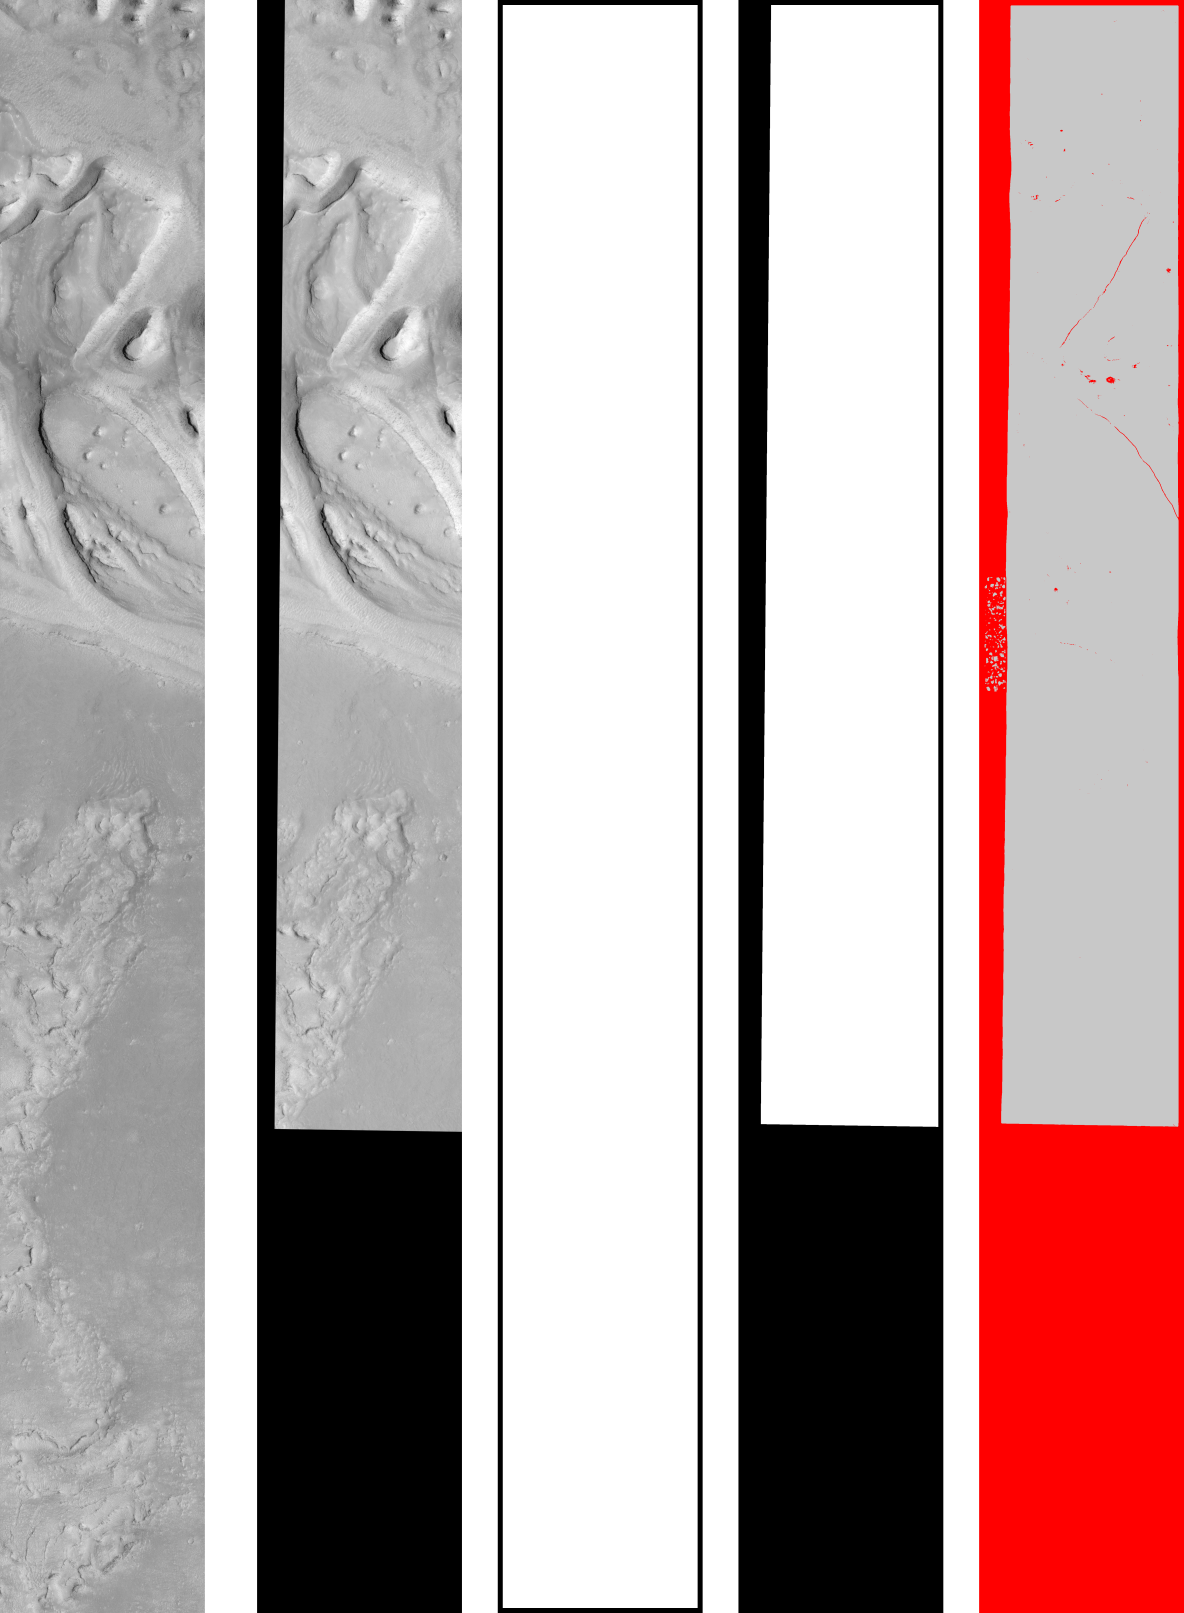
\includegraphics[width=4in]{images/p19-stereo-output.png}
\end{minipage}
\hfill
\begin{minipage}{2.9in}
\caption[P19 stereo output images]{
    \label{p19-stereo-output}
        These are the four viewable \texttt{.tif} files created by the
        \texttt{stereo} program.  On the left are the two aligned,
        pre-processed images: (\texttt{E0201461-M0100115-L.tif} and
        \texttt{E0201461-M0100115-R.tif}).  The next two are mask images
        (\texttt{E0201461-M0100115-lMask.tif} and
        \texttt{E0201461-M0100115-rMask.tif}), which indicate which
        pixels in the aligned images are good to use in stereo
        correlation.  The image on the right is the ``Good Pixel
        map'', (\texttt{E0201461-M0100115-GoodPixelMap.tif}), which
        indicates (in gray) which were successfully matched with the
        correlator, and (in red) those that were not matched.}
\end{minipage}
\end{figure}

Perhaps the most accessible file for assessing the quality of your
results is the good pixel image,
\\ (\texttt{E0201461-M0100115-GoodPixelMap.tif}).  If this file shows
mostly good, gray pixels in the overlap area (the area that is white
in both the \texttt{E0201461-M0100115-lMask.tif} and
\texttt{E0201461-M0100115-rMask.tif} files), then your results are
just fine.  If the good pixel image shows lots of failed data,
signified by red pixels in the overlap area, then you need to go back
and tune your \texttt{stereo.default} file until your results improve.
This might be a good time to make a copy of \texttt{stereo.default} as
you tune the parameters to improve the results.

You should also know that whenever the \texttt{stereo} executable is
run, it makes a copy of the configuration file used in
\textit{output-prefix}-stereo.default. Opening that output file will
show when the command was run, what the flags were from the command
line, and then a copy of the \texttt{stereo.default}. This will
hopefully help debug and log what was performed so that others in the
future can recreate your work.

Another handy debugging tool is the \texttt{disparitydebug} program,
which allows you to generate viewable versions of the intermediate
results from the stereo correlation algorithm.
\texttt{disparitydebug} converts information in the disparity image
files into two TIFF images that contain horizontal and vertical
components of the disparity (i.e. matching offsets for each pixel in
the horizontal and vertical directions).  There are actually three
flavors of disparity map: the \texttt{-D.tif}, the \texttt{-RD.tif},
and \texttt{-F.tif}.  You can run \texttt{disparitydebug} on any of
them.  Each shows the disparity map at the different stages of
processing.

\begin{verbatim}
    ISIS 3> cd results
    ISIS 3> disparitydebug E0201461-M0100115-F.tif
\end{verbatim}

If the output H and V files from \texttt{disparitydebug} look okay,
then the point cloud image is most likely ready for post-processing.
You can proceed to make a mesh or a \ac{DEM} by processing
\texttt{E0201461-M0100115-PC.tif} using the \texttt{point2mesh} or
\texttt{point2dem} tools, respectively.

\begin{figure}[b!]
\begin{minipage}{4in}
\includegraphics[width=4in]{images/p19-disparity.png}
\end{minipage}
\hfill
\begin{minipage}{2.7in}
\caption[P19 disparity images]{
    \label{p19-disparity}
	Disparity images produced using the \texttt{disparitydebug}
        tool.  The two images on the left are the
        \texttt{E0201461-M0100115-D-H.tif} and
        \texttt{E0201461-M0100115-D-V.tif} files, which are normalized
        horizontal and vertical disparity components produced by the
        disparity map initialization phase.  The two images on the
        right are \texttt{E0201461-M0100115-F-H.tif} and
        \texttt{E0201461-M0100115-F-V.tif}, which are the final
        filtered, sub-pixel-refined disparity maps that are fed into the
        Triangulation phase to build the point cloud image.  Since
        these MOC images were acquired by rolling the spacecraft
        across-track, most of the disparity that represents topography
        is present in the horizontal disparity map.  The vertical
        disparity map shows disparity due to ``wash-boarding,'' which
        is not from topography but from spacecraft movement. Note
        however that the horizontal and vertical disparity images are
        normalized independently.  Although both have the same range
        of gray values from white to black, they represent
        significantly different absolute ranges of disparity.}
\end{minipage}
\end{figure}

\clearpage

\section{Visualizing and Manipulating the Results}
\label{visualising}

When \texttt{stereo} finishes, it will have produced a point cloud
image.  At this point, many kinds of data products can be built from
the \texttt{E0201461-M0100115-PC.tif} point cloud file.

\subsection{Building a 3D Model}

If you wish to see the data in an interactive 3D browser, then you can
generate a 3D object file using the \texttt{point2mesh} command (page
\pageref{point2mesh}). The resulting file is stored in Open Scene
Graph binary format \cite{OSG_website}.  It can be viewed with
\texttt{osgviewer} (the Open Scene Graph Viewer program, distributed
with the binary version of the Stereo Pipeline).  The
\texttt{point2mesh} program takes the point cloud file and the left
normalized image as inputs:

\begin{verbatim}
    ISIS 3> point2mesh E0201461-M0100115-PC.tif E0201461-M0100115-L.tif -l
\end{verbatim}

\noindent
When the \texttt{osgviewer} program starts, you may want to toggle the
lighting with the `L' key, toggle texturing with the 'T' key, and
toggle wireframe mode with the 'W'.  Press '?' to see a variety of
other interactive options.

\begin{figure}[h!]
\begin{minipage}{5in}
\includegraphics[width=5in]{images/p19-osg.png}
\end{minipage}
\hfill
\begin{minipage}{1.7in}
\caption[P19 in OSG]{
    \label{p19-osg}
	The \texttt{E0201461-M0100115.ive} file displayed in the OSG
        Viewer.  }
\end{minipage}
\end{figure}

\subsection{Building a Digital Elevation Model}

The \texttt{point2dem} program (page \pageref{point2dem}) creates a
Digital Elevation Model (\ac{DEM}) from the point cloud file.

\begin{verbatim}
    ISIS 3> point2dem E0201461-M0100115-PC.tif
\end{verbatim}

\noindent
The resulting TIFF file is map projected and will contain
georeferencing information stored as GeoTIFF tags. You can specify a
coordinate system (e.g., mercator, sinusoidal) and a reference
spheroid (i.e., calculated for the Moon or Mars).

\begin{verbatim}
    ISIS 3> point2dem -r mars E0201461-M0100115-PC.tif
\end{verbatim}

\noindent
This product is suitable for scientific use, and can be imported into
a variety of GIS platforms.  However, the resulting file,
\texttt{E0201461-M0100115-DEM.tif}, will have 32-bit floating point
pixels, and will not render well in typical image viewers.

The \texttt{point2dem} program can also be used to orthoproject raw
satellite imagery onto the \ac{DEM}. To do this, invoke
\texttt{point2dem} just as before, but add the \texttt{-\/-orthoimage}
option and specify the use of the left image file as the texture file
to use for the projection:

\begin{verbatim}
    ISIS 3> point2dem -r mars --orthoimage E0201461-M0100115-L.tif \
        E0201461-M0100115-PC.tif
\end{verbatim}

\noindent
The \texttt{point2dem} program is also able to accept output
projection options the same way as the tools in GDAL. Well known EPSG,
IAU2000 projections, and custom Proj4 strings can applied with the
target spatial reference set flag, \texttt{-\/-t\_srs}. If the target
spatial reference flag is applied with any of the reference spheroid
options, the reference spheroid option will overwrite the datum
defined in the target spatial reference set. The following examples
produce the same output.

\begin {verbatim}
    ISIS 3> point2dem --t_srs IAU2000:49900 E0201461-M0100115-PC.tif
    ISIS 3> point2dem --t_srs "+proj=longlat +a=3396190 +b=3376200"
        E0201461-M0100115-PC.tif
\end{verbatim}

\noindent
The \texttt{point2dem} program can be used in many different ways.  Be
sure to take your time to explore all of the options.

\begin{figure}
\hfill
\begin{minipage}{3.5in}
\includegraphics[width=3.5in]{images/p19-norm_ortho.png}
\end{minipage}
\hfill
\begin{minipage}{2in}
\caption[P19 Normalized DEM and Orthophoto]{
    \label{p19-norm_ortho}
	The image on the left is a normalized DEM (generated using the
        \texttt{-n} option), which shows low terrain values as black
        and high terrain values as white.  The image on the right is
        the left input image projected onto the DEM (created using the
        \texttt{-\/-orthoimage} option to \texttt{point2dem}).  }
\end{minipage}
\hfill
\end{figure}

% \begin{figure}
% \begin{center}
% \includegraphics[width=4in]{images/p19-dems.png}
% \caption[P19 dem images]{
%     \label{p19-dems}
%	The non-normalized and normalized DEMs. Note that the
%	non-normalized version contains floating point pixel values
%	and will not open in most image viewing programs which
%	expect integer pixel values between 0 and 255 (which is
%	what the normalized version does for you).
%     }
% \end{center}
% \end{figure}
%
% \begin{figure}
% \begin{center}
% 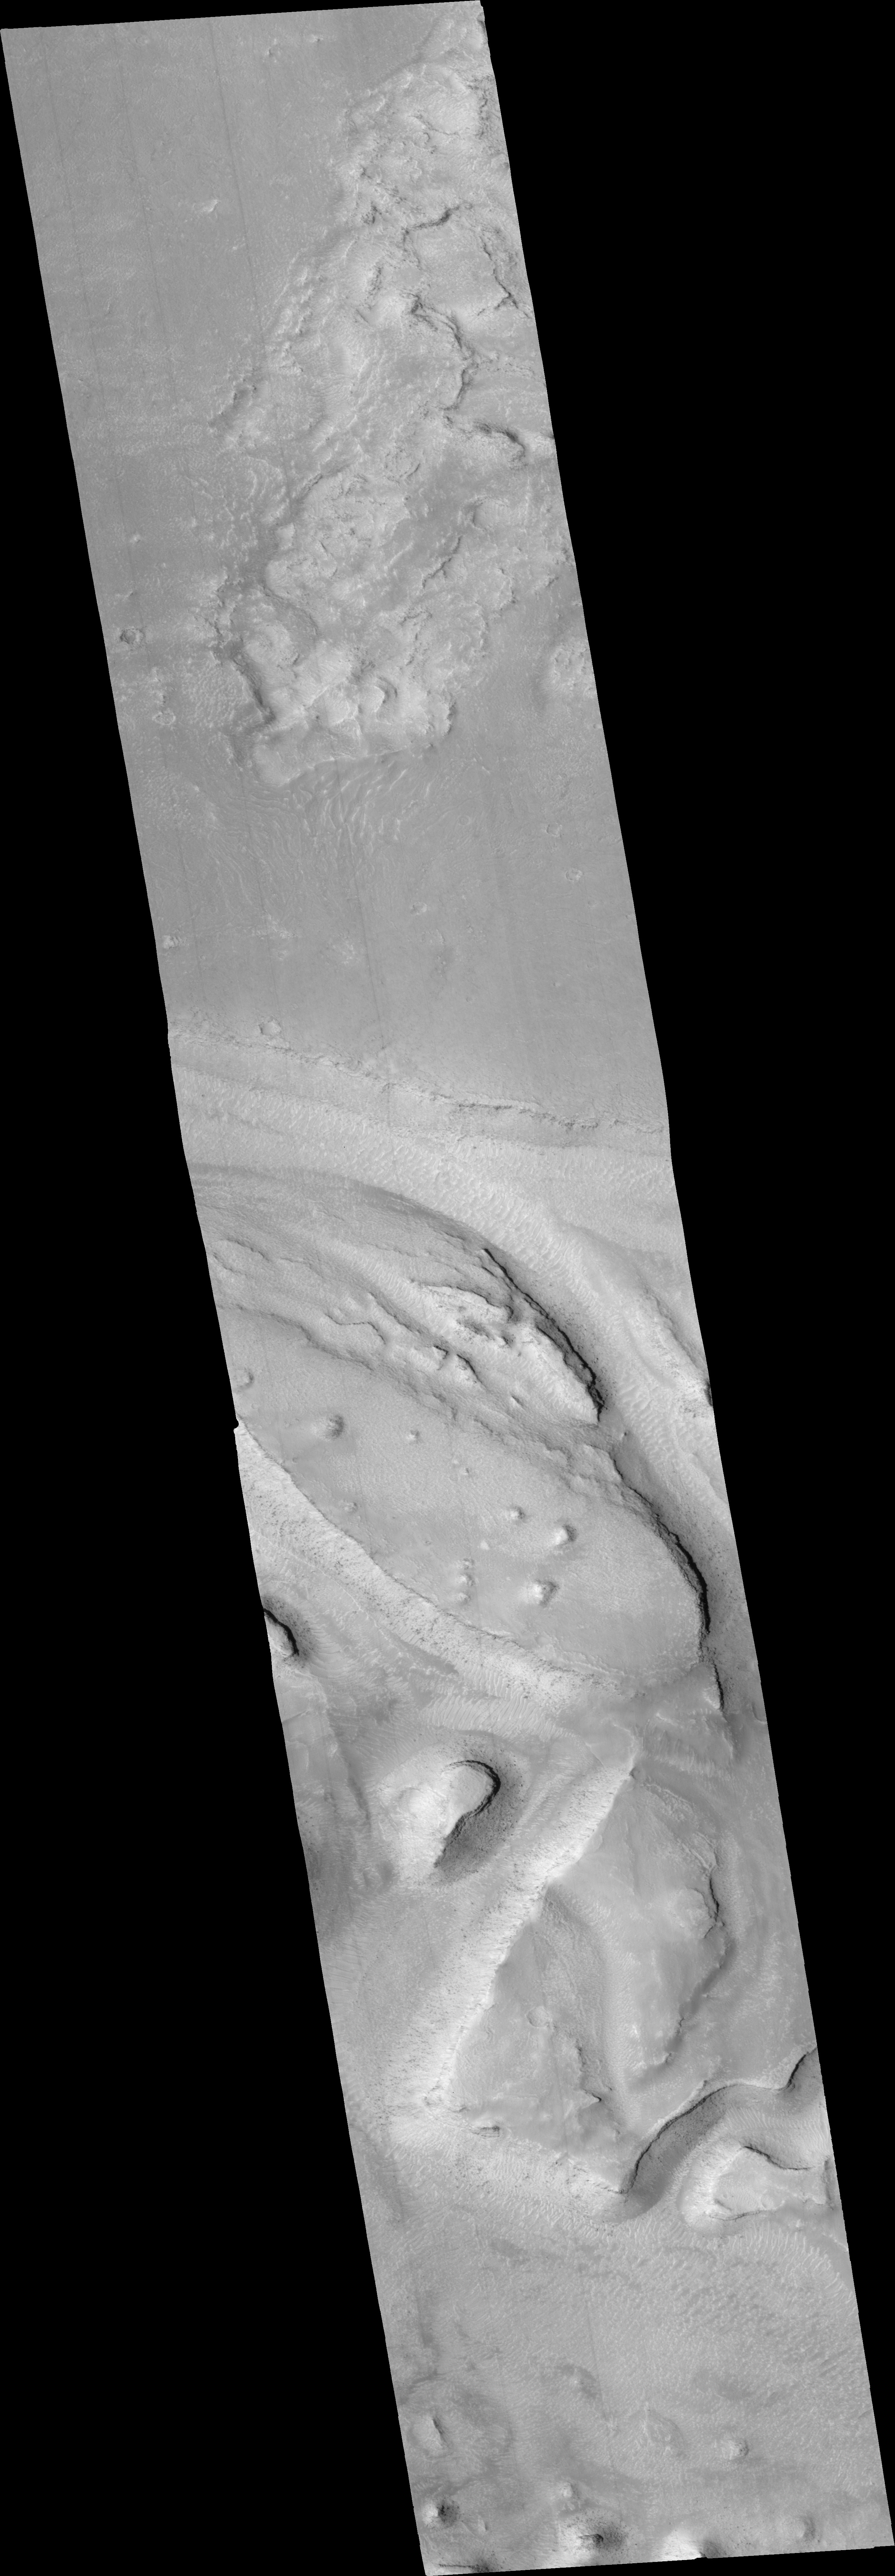
\includegraphics[width=3in]{images/p19-ortho.png}
% \caption[P19 orthophoto]{
%     \label{p19-ortho}
%	The left image orthoprojected onto the DEM.
%     }
% \end{center}
% \end{figure}

\clearpage

\subsection{Creating DEMs relative to the Geoid/Areoid}

The DEMs generated using \texttt{point2dem} are in reference to a datum
ellipsoid. If desired, the \texttt{dem\_geoid} program can be used to
convert this DEM to be relative to a geoid/areoid on Earth/Mars
respectively.

\subsection{Converting to the LAS Format}

If it is desired to use the generated point cloud in contexts outside
ASP, it can be converted to the LAS file format, which is a public file
format for the interchange of 3-dimensional point cloud data. The tool
\texttt{point2las} can be used for that purpose (section \ref{point2las}).

\subsection{Generating Color Hillshade Maps}

Once you have generated a \ac{DEM} file, you can use the Vision Workbench's
\texttt{colormap} and \texttt{hillshade} tools to create colorized
and/or shaded relief images.

To create a colorized version of the \ac{DEM}, you need only specify
the \ac{DEM} file to use. The colormap is applied to the full range of
the DEM, which is computed automatically.  Alternatively you can
specific your own min and max range for the color map.

\begin{verbatim}
    ISIS 3> colormap E0201461-M0100115-DEM.tif -o hrad-colorized.tif
\end{verbatim}

To create a hillshade of the \ac{DEM}, specify the \ac{DEM} file to
use. You can control the azimuth and elevation of the light source
using the \texttt{-a} and \texttt{-e} options.

\begin{verbatim}
    ISIS 3> hillshade E0201461-M0100115-DEM.tif -o hrad-shaded.tif -e 25
\end{verbatim}

To create a colorized version of the shaded relief file, specify
the \ac{DEM} and the shaded relief file that should be used:

\begin{verbatim}
    ISIS 3> colormap E0201461-M0100115-DEM.tif -s hrad-shaded.tif -o hrad-color-shaded.tif
\end{verbatim}

\begin{figure}[b!]
\begin{center}
\includegraphics[width=4.7in]{images/p19-colorized-shaded.png}
\caption[Hrad colorized and shaded relief]{
    \label{hrad-color}
	The colorized DEM, the shaded relief image, and the colorized hillshade.
    }
\end{center}
\end{figure}

\clearpage

\subsection{Building Overlays for Moon and Mars mode in Google Earth}

The final program in the Stereo Pipeline package that this tutorial
will address is \texttt{image2qtree}.  This tool was designed to
create tiled, multi-resolution overlays for Google Earth.  In addition
to generating image tiles, it produces a metadata tree in KML format
that can be loaded from your local hard drive or streamed from a
remote server over the Internet.

The \texttt{image2qtree} program can only be used on 8-bit image files
with georeferencing information (e.g. grayscale or RGB geotiff
images). In this example, it can be used to process \\
\texttt{E0201461-M0100115-DEM-normalized.tif},
\texttt{E0201461-M0100115-DRG.tif} \texttt{hrad-shaded.tif}, \\
\texttt{hrad-colorized.tif}, and \texttt{hrad-shaded-colorized.tif}

\begin{verbatim}
    ISIS 3> image2qtree hrad-shaded-colorized.tif -m kml --draw-order 100
\end{verbatim}

\begin{figure}[b!]
\begin{center}
\includegraphics[width=6in]{images/p19-googlemars.png}
\caption[Hrad shaded colorized DEM as a KML overlay] {
    \label{hrad-kml}
        The colorized hillshade DEM as a KML overlay.  }
\end{center}
\end{figure}


\part{The Stereo Pipeline in Depth}
\chapter{Correlation}
\label{ch:correlation}



The entire stereo correlation process, from raw input images to a
point cloud or DEM, can be viewed as a multistage pipeline as depicted
in Figure~\ref{fig:asp}.

\begin{figure}[tb]
  \centering
%  \includegraphics[width=7cm]{images/asp}
  \caption{Flow of data through the Ames Stereo Pipeline}
  \label{fig:asp}
\end{figure}

The process begins with least squares Bundle Adjustment, which is
described in Section~\ref{sec:bundle_adjustment}, below.  This
produces corrected extrinsic camera parameters that are utilized by
various camera modeling steps.

Then, the left and right images are aligned using interest points or
geometric constraints from the camera models.  This step is often
essential for performance because it ensures that the disparity search
space is bounded to a known area.  Next, a prepossessing filter such
as the Sign of the Laplacian of the Gaussian filter is used, which has
the effect of producing images that are somewhat invariant to
differences in lighting conditions~\cite{Nishihara84practical}.

Following these pre-processing steps, we compute the disparity space
image $DSI(i,j,d_x, d_y)$ that stores the matching cost between a left
image block centered around pixel $(i,j)$ and a right image block
centered at position $(i-d_x, j-d_y)$.  At this stage, the quality of
the match is measured as the normalized cross
correlation~\cite{Menard97:robust} between two 15x15 pixel image
patches.  We employ several optimizations to accelerate this
computation: (1) a box filter-like accumulator that reduces duplicate
operations in the calculation of $DSI$~\cite{Sun02rectangular}; (2) a
coarse-to-fine pyramid based approach where disparities are estimated
using low resolution images, and then successively refined at higher
resolutions; and (3) partitioning of the disparity search space into
rectangular sub-regions with similar values of disparity determined in
the previous lower resolution level of the
pyramid~\cite{Sun02rectangular}.

The $DSI$ estimate just described efficiently computes {\em integer}
estimates of disparity between the two images.  These estimates are
subsequently refined to sub-pixel accuracy using the technique
described in Section~\ref{sec:subpixel}.  Finally, in conjunction with
the bundle adjusted camera models, the sub-pixel disparity estimates
are used to triangulate the location of 3D points as the closest point
of intersection of two forward-projected rays emanating from the
centers of the two cameras through the matched pixels.


\section{Sub-pixel Stereo Correlation}\label{sec:subpixel}

Apollo images are affected by two types of noise inherent to the
scanning process: (1) the presence of film grain and (2) dust \& lint
particles.  The former gives rise to noise in the DEM values that wash
out real features, and the latter causes incorrect matches or hard to
detect blemishes in the DEM.  Attenuating the effect of these scanning
artifacts while simultaneously refining the integer disparity map to
sub-pixel accuracy has become a critical goal of our system, and is
necessary for processing real-world data sets such as the Apollo
Metric Camera data.

A common technique in sub-pixel refinement is to fit a parabola to the
correlation cost surface in the 8-connected neighborhood around the
integer disparity estimate, and then use the parabola's minimum as the
sub-pixel disparity value. This method is easy to implement and fast
to compute, but exhibits a problem known as pixel-locking: the
sub-pixel disparities tend toward their integer estimates and can
create noticable "stair steps" on surfaces that should be
smooth~\cite{Stein06:attenuating},~\cite{Szeliski03sampling}.  One way
of attenuating the pixel-locking effect is through the use of a
symmetric cost function~\cite{Nehab05:improved} for matching the
``left'' and ``right'' image blocks.  

To avoid the high computational complexity of these methods another
class of approaches based on the Lucas-Kanade
algorithm~\cite{Baker04:lucas-kanade} proposes an asymmetric score
where the disparity map is computed using the best matching score
between the left image block and an optimally affine transformed block
from the right image.  For example, the sub-pixel refinement developed
by Stein et. al.~\cite{Stein06:attenuating} lets $I_R(m,n)$ and
$I_L(i,j)$ be two corresponding pixels in the right and left image
respectively, where $i = m+d_x$, $j = n+d_y$ and $d_x, d_y$ are the
integer disparities.  They develop a linear approximation based on the
Taylor Series expansion around pixel $(i,j)$ in the left image
\begin{eqnarray}
I_L(i+\delta_x,j + \delta_y)\approx I_L(i,j) + \delta_x\frac{dI_L}{d_x}(i,j)+\delta_y\frac{dI_L}{d_y}(i,j) 
\label{taylor_expansion}
\end {eqnarray}
where $\delta_x$ and $\delta_y$ are the local sub-pixel displacements.
Let $e(x,y) = I_R(x,y) - I_L(i+\delta_x,j+\delta_y)$ and $W$ be an
image window centered around pixel $(m,n)$.  The local displacements
are not constant accross $W$ and they vary according to:
\begin{eqnarray}
\nonumber
\delta_x(i,j) = a_1i+b_1j+c_1\\
\delta_y(i,j) = a_2i+b_2j+c_2. 
\label{affine_transform}
\end {eqnarray}
The goal is to find the parameters $a_1, b_1, c_1, a_2, b_2, c_2$ that
minimize the cost function
\begin{eqnarray}
{\bf E}(m,n) =\sum_{(x,y)\in W} (e(x,y)w(x,y))^2
\label{affine2D_cost}
\end{eqnarray}
where $w(x,y)$ are a set of weights used to reject outliers. Note that
the local displacements $\delta_x(i,j)$ and $\delta_y(i,j)$ depend on
the pixel positions within the window $W$. In fact, the values $a_1,
b_1, c_1, a_2, b_2, c_2$ that minimize $\bf E$ can be seen as the
parameters of an affine transformation that best transforms the right
image window to match the reference (left) image window.

%In the original Lucas-Kanade method the weights are set
%$w(x,y)=1$. In~\cite{Stein06:attenuating} the values the weights
%$w(x,y)$ determined heuristically to reject the noise and emphasize
%the pixel closer to the center of the window. An alternative solution
%is to use a set of constant weights derived from the Cauchy
%distribution~\cite{Menard97:robust} given by: \begin{eqnarray}
%w(x,y)= \frac{\sqrt{b^2 \log(1+\frac{I_e^2(x,y)}{b^2})}
%}{|I_e(x,y)|} \label{Cauchy_weights} \end{eqnarray} where $b$ is some
%fixed threshold (in our experiments $b = 10^{-4}$) and $I_e(x,y) =
%I_R(x,y)-I_L(i,j)$.
 
%The steps of this method are given below
%\begin{itemize}
%\item {\bf Step 1:} Compute $\frac{dI_L}{d_x}(i,j)$, $\frac{dI_L}{d_y}(i,j)$ and the $I_R(x,y)$ values using bilinear interpolation. Initialize the parameters $a_1, b_1, c_1, a_2, b_2, c_2$.
%\item {\bf Step 2:} Determine ${a_1, b_1, c_1, a_2, b_2, c_2}$ to minimize ${\bf E}$. 
%\item {\bf Step 3:} Compute $\delta_x(i,j)$ and $\delta_y(i,j)$ using Equation~\ref{affine_transform}.
%\item {\bf Step 4:} Compute a new point $(x', y') = (x, y) + (\delta_x, \delta_y)$ and the $I_R(x',y')$ values using bilinear interpolation.
%\item {\bf Step 5:} Check for convergence. If norm of ($\delta_x, \delta_y$) vector falls below a fixed threshold the iterations converged. Otherwise, go to step 1.
%\end{itemize}

The shortcoming of this method is directly related to the cost
function that it is minimizing, which has a low tolerance to noise.
Noise present in the image will easily dominate the result of the
squared error function, giving rise to erroneous disparity
information.  Recently, several statistical
approaches (e.g. ~\cite{cheng04:bayesian}) have emerged to show how
stochastic models can be used to attenuate the effects of noise.  Our
sub-pixel refinement technique~\cite{Nefian09:bayesian} adopts some of
these ideas, generalizing the earlier work by Stein
et. al.~\cite{Stein06:attenuating} to a Bayesian framework that models
both the data and image noise.

%\begin{eqnarray}
%\nonumber
%{\bf E}(m,n))&=& \sum_{(x,y)\in W}((I_R(x,y) - I_L(i+\delta_x, j+\delta_y))^2\\
%\nonumber
%\tilde{\delta_x} &=& \arg \min_{\delta_x} {\bf E}(m,n)\\
%\nonumber
%\tilde{\delta_y} &=& \arg \min_{\delta_x} {\bf E}(m,n)\\
%\nonumber           
%P({\bf I}_R(m,n))&=&\prod_{(x,y)\in W}{\cal N}(I_R(x,y)|I_L(i+\delta_x, j+\delta_y), \sigma_p)P(k=0)\\
%\nonumber
%                 &+&{\cal N}(I_R(x,y)|\mu_n, \sigma_n)P(k=1)\\
%\nonumber
%\tilde{\delta_x} &=& \arg \max_{\delta_x} P({\bf I}_R(m,n))\\
%\nonumber
%\tilde{\delta_y} &=& \arg \max_{\delta_y} P({\bf I}_R(m,n))\\
%\nonumber
%m &=& m+\tilde{\delta_x}\\
%\nonumber
%n &=& n+\tilde{\delta_y}
%\end{eqnarray}

In our approach the probability of a pixel in the right image is given
by the following Bayesian model:
\begin{eqnarray}
P(I_R(m,n))&=& \prod_{(x,y)\in W}{\cal N}(I_R(m,n)|I_L(i+\delta_x, j+\delta_y), \frac{\sigma_p}{\sqrt{g_{xy}}})P(z=0) + \\
\nonumber
           &+& {\cal N}(I_R(m,n)|\mu_n, \sigma_n)P(z=1)
\label{pix}
\end {eqnarray}
The first mixture component $(z=0)$ is a normal density function with
mean $I_L(i+\delta_x, j+\delta_y)$ and variance $\frac{\sigma_p}{\sqrt{g_{xy}}}$:
\begin{eqnarray}
P(I_R(m,n)|z=0) = {\cal N}(I_R(m,n)|I_L(i+\delta_x, j+\delta_y), \frac{\sigma_p}{\sqrt{g_{xy}}})
\label{pixel_stereo_model}
\end {eqnarray}
The $\frac{1}{\sqrt{g_{xy}}}$ factor in the variance of this component
has the effect of a Gaussian smoothing window over the patch. With
this term in place, we are no longer looking for a single variance
over the whole patch; instead we are assuming the variance increases
with distance away from the center according to the inverted Gaussian,
and are attempting to fit a global scale, $\sigma_p$. This provides
formal justification for the standard Gaussian windowing kernel.

The second mixture component $(z=1)$ in
Equation~\ref{pixel_stereo_model} models the image noise using a
normal density function with mean $\mu_n$ and variance $\sigma_n$:
\begin{eqnarray}
P(I_R(m,n)|z=1) = {\cal N}(I_R(m,n)|\mu_n, \sigma_n)
\label{pixel_noise_model}
\end {eqnarray}
Let ${\bf I}_R(m,n)$ be a vector of all pixels values in a window $W$
centered in pixel $(m,n)$ in the right image. Then,
\begin{eqnarray}
P({\bf I}_R(m,n)) = \prod_{(x,y)\in W}P(I_R(x,y))
\label{bayes_model}
\end {eqnarray}

The parameters $\lambda = \{a_1, b_1, c_1, a_2, b_2, c_2,
\sigma_p,\mu_n, \sigma_n\}$ that maximize the model likelihood in
Equation~\ref{bayes_model} are determined using the Expectation
Maximization (EM) algorithm. Maximizing the model likelihood in
Equation~\ref{bayes_model} is equivalent to maximizing the auxiliary
function:
\begin{eqnarray}
\nonumber
{\bf Q(\theta)}&=& \sum_k P(k|{\bf I}_R, \lambda_t) \log P ({\bf I}_R, k, {\underline \delta}|\lambda)\\
&=& \sum_{k}\sum_{x,y} P(k|I_R(x,y), \lambda_t)\log P (I_R(x,y)|k, \lambda)P(k|\lambda)
\label{aux_function}
\end {eqnarray}

Note that the M step calculations are similar to the equation used to
determine the parameters $a_1, b_1, c_1, a_2, b_2, c_2$ in the method
presented in~\cite{Stein06:attenuating}, except here the fixed set of
weights is replaced by the a posteriori probabilities computed in the
E step. In this way, our approach can be seen as a generalization of
the Lucas-Kanade method.  The complete algorithm is summarized in the following steps:
\begin{itemize}
\item {\bf Step 1:} Compute $\frac{dI_L}{d_x}(i,j)$, $\frac{dI_L}{d_y}(i,j)$ and the $I_R(x,y)$ values using bilinear interpolation. Initialize the model parameters $\lambda$.
\item {\bf Step 2:} Compute iteratively the model parameters $\lambda$ using the EM algorithm (see ~\cite{Nefian09:bayesian} for details). 
\item {\bf Step 3:} Compute $\delta_x(i,j)$ and $\delta_y(i,j)$ using Equation~\ref{affine_transform}.
\item {\bf Step 4:} Compute a new point $(x', y') = (x, y) + (\delta_x, \delta_y)$ and the $I_R(x',y')$ values using bilinear interpolation.
\item {\bf Step 5:} If the norm of ($\delta_x, \delta_y$) vector falls below a fixed threshold the iterations converged. Otherwise, go to step 1.
\end{itemize}

\begin{figure}[bt]
  \begin{center}
%    \subfigure[]{\includegraphics[width=6cm]{images/orbit33}}
%    \subfigure[]{\includegraphics[width=6cm]{images/apollo_3D}}
    \caption{Hadley Rille and the Apollo 15 landing site derived from
      Apollo Metric Camera frames AS15-M-1135 and AS15-M-1136. (a)
      superimposed over the USGS Clementine base map, (b) oblique view.}
    \label{results_crater_img}
  \end{center}
\end{figure} 

Like the computation of the integer $DSI$, we adopt a multi-scale
approach for sub-pixel refinement. At each level of the pyramid, the
algorithm is initialized with the disparity determined in the previous
lower resolution level of the pyramid. This allows the subpixel
algorithm to shift the results of the integer $DSI$ by many pixel if
a better match can be found using the affine, noise-adapted window.


%-----

This chapter provides a graphical representation of how correlation is
performed in Ames Stereo Pipeline. Most importantly this provides a
quick comparison of different algorithms provided to save the user the
time of comparing results themselves.

For this chapter we'll be using the north most tip of Hadley Rille as
captured by the Apollo 15 Metric Camera. Here's what the left and right
pair looks like before any processing has been applied. The right image
is actually larger than the left.

\begin{figure}[hb]
\centering
  \subfigure[{\tt Left}]{\includegraphics[width=3in]{images/correlation/sub4-AS15-M-1134_crop.png}\label{fig:left_input_image}}
  \hfil
  \subfigure[{\tt Right}]{\includegraphics[width=3in]{images/correlation/sub4-AS15-M-1135_crop.png}\label{fig:right_input_image}}
\caption{Original input images used for this chapter.}
\label{fig:input_images}
\end{figure}

\section{Preprocessing Filters and Integer Correlation}
\label{sec:prefilter_n_correlation}

\subsection{Cost Functions}

\subsection{Gaussian Blur}

\subsection{Log Filter}

\subsection{SLog Filter}

\subsection{Pyramid Correlator}

\section{Sub-pixel Correlation}
\label{sec:subpixel_correlation}

\subsection{Parabola}

\begin{figure}[hb]
\centering
  \subfigure[{\tt 3D result}]{\includegraphics[width=3in]{images/correlation/3D_mode0.png}}
  \hfil
  \subfigure[{\tt Hillshade Result}]{\includegraphics[width=3in]{images/correlation/hillshade_mode0.png}}
\caption{Results using Parabola subpixel mode.}
\label{fig:parabola_results}
\end{figure}

\subsection{Robust weighted Affine}

\begin{figure}[hb]
\centering
  \subfigure[{\tt 3D result}]{\includegraphics[width=3in]{images/correlation/3D_mode1.png}}
  \hfil
  \subfigure[{\tt Hillshade Result}]{\includegraphics[width=3in]{images/correlation/hillshade_mode1.png}}
\caption{Results using Robust Affine subpixel mode.}
\label{fig:robust_results}
\end{figure}

\subsection{Bayes weighted Affine}

\begin{figure}[hb]
\centering
  \subfigure[{\tt 3D result}]{\includegraphics[width=3in]{images/correlation/3D_mode2.png}}
  \hfil
  \subfigure[{\tt Hillshade Result}]{\includegraphics[width=3in]{images/correlation/hillshade_mode2.png}}
\caption{Results using Bayes weighted Affine subpixel mode.}
\label{fig:bayes_results}
\end{figure}

\subsection{Bayes EM weighted Affine}

\begin{figure}[hb]
\centering
  \subfigure[{\tt 3D result}]{\includegraphics[width=3in]{images/correlation/3D_mode3.png}}
  \hfil
  \subfigure[{\tt Hillshade Result}]{\includegraphics[width=3in]{images/correlation/hillshade_mode3.png}}
\caption{Results using Bayes EM weighted Affine subpixel mode.}
\label{fig:bayes_em_results}
\end{figure}

\chapter{Bundle Adjustment}

Bundle adjustment is the process of simultaneously adjusting the
properties of multiple cameras and the 3D locations of the objects
they see, to minimize the error between the estimated forward
projection of the 3D objects and their measured location in the captured
images. 

\begin{figure}[htp]
  \begin{center}
  \includegraphics[trim=20mm 20mm 20mm 15mm,clip,width=6in]{images/ba_feature_observation.pdf}
  \end{center}
  \caption{ A feature observation in Bundle Adjustment. \cite{moore09} }
  \label{fig:ba_feature}
\end{figure}

This has application as an optional step between the capture
of images and the creation of DEMs. There is always an amount of error
with the recorded position and orientation of cameras and Bundle
Adjustment can be used to refine these measurements. This will allow
DEMs from multiple cameras to align better with one another. Bundle
Adjustment can also take advantage of Ground Control Points (GCPs),
which are accurately measured 3D locations on the surface of the DEM. GCPs
can be used to improve the alignment of the DEMs or align the new DEM
to a past data product. Finally, even though Bundle Adjustment
calculates the location of the 3D objects it views, only the final
properties of cameras are recorded in the Ames Stereo Pipeline. Those
properties are loaded into \texttt{stereo} which will then use it's own
method for triangulation.

\subsection{A deeper understanding}

Bundle Adjustment in Ames Stereo Pipeline revolves around the
Levenberg-Marquardt Algorithm (LMA) which is a method for minimizing a
function. In the case of Bundle Adjustment, the error $\epsilon$ is
the pixel difference between an objects location in an image,
$[u_{f},v_{f}]$, and it's forward projection through the camera,
$[\tilde{u}_{f},\tilde{v}_{f}]$. The goal is to solve for an update to
the parameters of the cameras and point positions, apply them, and
then repeat until the update supplied by LMA goes to zero. The
equation for LMA is below:

\begin{equation}
\mbox{\boldmath$\delta$} = \frac{\mbox{\boldmath$J^T\epsilon$}}{\bf{J^TJ}+\lambda\bf{I}}
\label{eqn: Levenberg-Marquardt Algorithm}
\end{equation}

LMA is a hybrid of two minimization techniques, gauss-newton and
gradient decent. Where the control between these two methods is the
parameter $\lambda$ which will change in value during the process of
Bundle Adjustment. A high value of $\lambda$ forces LMA to act like
gradient decent, and is what will happen at the beginning of bundle
adjustment when the camera parameters are far away from their final
solution. A low value of $\lambda$ drives LMA into the gauss-newton
method; at which it will take small steps in updating the camera
values. When Bundle Adjustment is almost finished and is close to the
solution, it will lower $\lambda$.

Since Bundle Adjustment is an iterative method, it would be happy to
keep processing new updates to camera parameters all day. To avoid
this, there are several shut-off conditions. The first is when the
update {\boldmath$\delta$} becomes insignificantly small. The second
is when the error measurement, {\boldmath$\epsilon$}, becomes
insignificantly small. Both of these conditions' thresholds are
defined within the bundle adjuster's code and is not allowed for the
user to change. The final shut off condition is when the number of
iterations becomes too large. It is important to understand that when
this shut off condition happens, bundle adjustment has not finished
refining the parameters of the cameras but they are a step closer to
the solution. The maximum number of iterations is changeable by the
user so they can decide how much time they're will to dedicate to the
correction of the data. The number of iterations Bundle Adjustment
takes to converge on the solution can be anywhere between 20
iterations to several hundred.

If you are interested in more information on the math of Bundle
Adjustment and the arrangement of the problem, we recommend reading
Appendix 6 in the {\em Multiple View Geometry} \cite{hartley04}.
For more information on why LMA is used instead of the many other
optimization algorithms, try reading {\em Bundle Adjustment – A Modern
Synthesis} \cite{triggs00}.

\section{ISIS Adjust}

The \texttt{isis\_adjust} program is an application designed to
perform bundle adjustment on the cameras supported by USGS's
ISIS3. \texttt{isis\_adjust} is special in that it does not
discriminate based on camera type. It can perform bundle adjustment on
line-scan imagers (such as MOC and Apollo's Panoramic Camera) just as
well as it can on traditional frame cameras (such as Apollo Metric
Camera). Theoretically it should also work fine with push-frame
imagers (i.e. video), though this is untested.

\texttt{isis\_adjust} works by first converting all pixel measurements
in an images to measurements defined on the ideal focal
plane using millimeters and the ephemeris time (ET). The ET is the
absolute second at which that pixel measurement was recorded on the camera. 
For a frame camera, the ET won't change for the for
any of the measurements on the image. For anything more exotic, it is
a different story. On a MOC image between the top and bottom line;
about 5 seconds could have passed.

\begin{wrapfigure}{r}{0.3\textwidth}
\vspace{-30pt}
\begin{center}
  \definecolor{lgray}{gray}{0.95}
  \fcolorbox{black}{lgray}{\begin{minipage}{0.29\textwidth} 

      \emph{Note from Author:} \\ Currently \texttt{isis\_adjust}
      lacks a proper way to support arbitrary defined correction
      functions. For the time being, \texttt{isis\_adjust} has been
      hard-coded to perform only zero order corrections (i.e. scalar
      offsets). (03/11/09)

  \end{minipage}}
\end{center}
\vspace{-30pt}
\end{wrapfigure}

When \texttt{isis\_adjust} calculates the partial derivatives of the
forward projection of a point, it will use an ideal pinhole camera
model. The properties of the ideal pinhole camera are defined as
properties of the subject camera at the specificed ET for the current
measure plus the correction function $f(t)$ that \texttt{isis\_adjust} is
solving for. $f(t)$ can be almost any function of ET, the only limit is the
number parameters in the equations. Some initial work hints that
anything greater than a $2^{nd}$ order polynomial becomes an ill-posed
problem.

\subsection{Options}

\begin{verbatim}
--cnet, -c [control network file]
\end{verbatim}

\emph{Optional.} Feeding this option will force ISIS Adjust to use an
already built control network. If not fed, ISIS Adjust will look for
match files in current operating directory with names similar to the
input images to build it's control network from. If
\texttt{isis\_adjust} creates it's own control network file, it will
save it as \verb=isis_adjust.cnet=.

\begin{verbatim}
--lambda, -l [value]
\end{verbatim}

\emph{Optional.} This set the starting value for $\lambda$. Bundle
Adjustment will naturally select a value for $\lambda$ it thinks is
best for the starting error, but this argument can be used to override
that. \emph{It's not recommended to change the starting value of
  $\lambda$ except for experienced users.}

\begin{verbatim}
--position-sigma [default = 100]
\end{verbatim}

Sets the sigma \emph{(uncertainty)} of the spacecraft position in
meters.

\begin{verbatim}
--pose-sigma [default = 0.1]
\end{verbatim}

Sets the sigma \emph{(uncertainty)} of the spacecraft pose in radians.

\begin{verbatim}
--gcp-sigma [default = 100]
\end{verbatim}

Sets the sigma \emph{(uncertainty)} of the ground control points in
meters.

\begin{verbatim}
--run-match, -m
\end{verbatim}

\emph{Optional.} If match files don't already exist, create them using a
call to \texttt{IPmatch}.

\begin{verbatim}
--match-debug-images, -d
\end{verbatim}

\emph{Optional.} If a call to \texttt{ipmatch} is being called, this option
also allows for the creation of debugging images that show the matches
between the input images.

\begin{verbatim}
--min-matches [default = 5]
\end{verbatim}

When producing a control network, this sets the minimum required
interest point matches between images for them to be included. If a
match file fails to find this many of matches, it probably means these
were poor matches and the images don't really overlap.

\begin{verbatim}
--max-iterations [default = 25]
\end{verbatim}

Sets the maximum number of iterations to be done by Bundle Adjustment.

\begin{verbatim}
--report-level, -r [default = 10]
\end{verbatim}

Sets the report level for the final report on the bundle adjustment
which can be found in \verb=rmax_adjust.report=. Report levels are defined in
BundleAdjustReport.h in Vision Workbench.

\begin{verbatim}
--nonsparse, -n
\end{verbatim}

\emph{Optional.} Switches the Bundle Adjustment code to use non-sparse
matrices in it's math. \emph{This will cause it to run significantly slower
and is only used as a check of the programmer's sparse matrix code.}

\begin{verbatim}
--write-isis-cnet-also
\end{verbatim}

\emph{Optional.} Write an ISIS PVL style control network file in
\verb=isis_adjust.net=. The output file is very large compared to the
binary output, \verb=isis_adjust.cnet=, and is human readable. This
alternative's importance is that it can be used with ISIS3's
\texttt{Qnet}.

\subsection{Examples of Use}

%\begin{wrapfigure}{r}{2.5in}
%\begin{center}
%  \definecolor{lgray}{gray}{0.95}
%  \fcolorbox{black}{lgray}{\begin{minipage}{2.2in} Hey! Hi we at IRG
%      actually use SURF! Blag sg f d fgds dfsgd srd sssf ds dfs fsdf
%      sd fdsrds rdsr drdf dgsrr ge gerges s i srges ge
%  \end{minipage}}
%\end{center}
%\end{wrapfigure}

What follows is an example of using two Mars Orbital Camera (MOC)
images of the south Cydonia region with \texttt{isis\_adjust}. We'll
be using images M10/00254 and R09/01059. These images are available
at Malin Space Science System's website
[\emph{http://www.msss.com/moc\_gallery/}] and at NASA's Planetary
Data System [\emph{http://pds.jpl.nasa.gov/index.shtml}]; be sure to
download the IMQ or IMG format. For reference, the following ISIS commands
are how to convert the MOC images to ISIS cubes.

\begin{verbatim}
        moc2isis from=m1000254.im? to=m1000254.lev0.cub
        moc2isis from=r0901059.im? to=r0901059.lev0.cub

        spiceinit from=m1000254.lev0.cub
        spiceinit from=r0901059.lev0.cub

        moccal from=m1000254.lev0.cub to=m1000254.cub
        moccal from=r0901059.lev0.cub to=r0901059.cub

        rm *.imq *.lev0.cub
\end{verbatim}

At this point a match file needs to be created that connects our to
cube files. Vision Workbench doesn't except cube files. So before
trying to match them; they'll have to be converted to a standard image
format.

\begin{verbatim}
        isis2std from=m1000254.cub to=m1000254.png format=PNG
        isis2std from=r0901059.cub to=r0901059.png format=PNG
\end{verbatim}

Here is how to process those newly created PNG files for interest points using the tools available in Vision Workbench.

\begin{verbatim}
        ipfind  m1000254.png r0901059.png
        ipmatch m1000254.png r0901059.png -d -r homography
\end{verbatim}

\definecolor{lgray}{gray}{0.95}
\begin{center}
\fcolorbox{black}{lgray}{ \begin{minipage}{5.5in} 

    \emph{Note from Author:} \\ Within IRG it has become apparent that
    using the interest point tools available from Vision Workbench
    does not produces enough matches to continue with Bundle
    Adjustment. The alternative is to use an outside method such as
    SURF \cite{surf09}. The trick is modifing an outside method's
    source code to export a Vision Workbench style match file. This
    can be difficult. Fortunately the patches to do this trick to the
    SURF code is available in the Appendix.  \\ \\ For this example it
    is okay to use the results from \texttt{ipfind} and
    \texttt{ipmatch}. Expect to find approximately 46 matched
    points. Your results will be slightly different due to the random
    nature of RANSAC.
\end{minipage}}
\end{center}

Finally, it is time to start Bundle Adjustment. There are many options
that can be done here. Below shows the options required to create
visualization data for \texttt{bundlevis} \emph{(This is covered in
  detail in the next section)}, setting the maximium iterations to
100, and finally the option to create a detailed report file of
\texttt{isis\_adjust}'s results.

\begin{verbatim}
        isis_adjust *.cub -s --max 100 -r 50
\end{verbatim}

The command window should spurt forth a lot of text and the directory
containing this project should suddenly have a lot more files. Don't
panic! This is perfectly normal! Looking through the output in the
terminal or alternatively in the output report file,
\verb=isis_adjust.report=, the problem should have convereged in 35
iterations. The error barely changed, this can be attributed Mars
Global Surveyor's relative positioning between images being very good. 

Producing DEMs using the newly created corrections is the same as
covered in Chapter 3. There is one fine difference in that
\texttt{stereo} needs to know of the existence of the correction
files, \verb=m1000254.isis_adjust= and
\verb=r0901059.isis_adjust=. Here is how that is done:

\begin{verbatim}
        stereo m1000254.cub r0901059.cub m1000254.isis_adjust
               r0901059.isis_adjust MOC_RESULTS/M1000254_R0901059
\end{verbatim}

\texttt{stereo} is excepting the correction files in the place where it would optionally accept a camera model file. It decides what to do with the input based on the file extension, in this case it is \verb=.isis_adjust=.

\section{Visualizing Bundle Adjustment with BundleVis}

Purpose, Examples, Supported Cameras, and File Types

\begin{figure}[htp]
  \begin{center}
  \includegraphics[width=6in]{images/bundlevis_apollo.png}
  \end{center}
  \caption{ A screenshot of bundle adjustment of Apollo 15's Orbit 33. }
  \label{fig:bundlevis}
\end{figure}

\begin{thebibliography}{1}

\bibitem{hartley04} Hartley, R.I. and Zisserman, A. ``Multiple View Geometry in Computer Vision,''
  Cambridge University Press. 2004. pp 597-627.
\bibitem{moore09} Moore, Wright, Schinstock, and Lewis. ``Comparison of Bundle Adjustment Formulations,''
  presented at ASPRS Annual Conf., Baltimore, Maryland, 2009.
\bibitem{triggs00} Triggs, McLauchlan, Hartley, and Fitzgibbon. ``Bundle Adjustment - A Modern Synthesis,''
  Lecture Notes in Computer Science. Vol. 1883, 298. January 2000
\bibitem{surf09} Bay, Gool, and Tuytelaars. (2009, Mar.). ``SURF: Speeded Up Robust Features'' [Online]. Available: \verb!http://www.vision.ee.ethz.ch/~surf/download.html!

\end{thebibliography}

%\include{data_visualization} <-- we should add this someday!
\chapter{Data Processing Examples}
\label{ch:examples}

\definecolor{lgray}{gray}{0.95}

This chapter showcases a variety of results that are possible when
processing different data sets with the Stereo Pipeline. It is also a
shortened guide that shows the commands used to process specific
mission data. There is no definitive method yet for making elevation
models as each stereo pair is unique. We hope that the following
sections serve as a cookbook for strategies that will get you started
in processing your own data. We recommend that you second check your
results against another source.

\section{Guidelines for Selecting Stereo Pairs}

When choosing image pairs to process, images that are taken with
similar viewing angles, lighting conditions, and significant surface
coverage overlap are best suited for creating terrain
models. Depending on the characteristics of the mission data set and
the individual images, the degree of acceptable variation will
differ. Significant differences between image characteristics
increases the likelihood of stereo matching error and artifacts, and
these errors will propagate through to the resulting data products.

Although images do not need to be map-projected before running the
\texttt{stereo} program, we recommend that you do run {\tt cam2map}
(or \texttt{cam2map4stereo.py})
beforehand, especially for image pairs that contain large topographic
variation (and therefore large disparity differences across the
scene, e.g., Valles Marineris).  Map-projection is especially necessary
when processing \ac{HiRISE} images. This removes the large disparity
differences between \ac{HiRISE} images and leaves only the small
detail for the Stereo Pipeline to compute. Remember that \ac{ISIS}
can work backwards through a map-projection when applying the camera
model, so the geometric integrity of your images will not be sacrificed
if you map-project first.

An alternative way of map-projection, that applies to non-ISIS imagery
as well, is with the \texttt{mapproject} tool (section
\ref{mapproj-example}).

Excessively noisy images will not correlate well, so images should be
photometrically calibrated in whatever fashion suits your purposes. If
there are photometric problems with the images, those photometric
defects can be misinterpreted as topography.

Remember, in order for \texttt{stereo} to process stereo pairs in
\ac{ISIS} cube format, the images must have had SPICE data associated
by running ISIS's \texttt{spiceinit} program run on them first.

%% \subsection{Comparing Examples to your System}

%% Since our first release we re-performed some of these examples and
%% recorded their processing time so you the user can judge how long it
%% will take you. Our examples were processed on our server called
%% `Lunokhod 2'. This server is a Dell PowerEdge Rack 900 purchased in
%% late 2009. Below are its specifications:

%% \begin{center}
%% \begin{tabular}{ l | l }
%% CPU & Dual E7420 Xeon at 2.13 GHz \emph{(16 logical cores)} \\ \hline
%% FSB & 1066 MHz \\ \hline
%% L2 Cache & 8 MB \\ \hline
%% Memory & 64 GB @ 667 MHz (mis-matched?) \\ \hline
%% Storage & Local RAID5 \\ \hline
%% OS & Red Hat Enterprise Linux 5.5 \\ \hline
%% BogoMIPS & 4256 \\ \hline
%% Color & Dell Graphite \\
%% \end{tabular}
%% \end{center}

%% The times recorded are listed in wall hours and CPU hours. Wall-hours
%% are how long it took the job to complete from the user's
%% perspective. CPU-hours are how much processing time it took to
%% complete. If the job took 30 wall-minutes on a 2 core system, it spent
%% 30 minutes in CPU 1 and CPU 2. Thus, the total CPU-hours would be
%% 1. This example, though correct, is not what always happens in the
%% real world. Inefficiency with managing multiple threads or the
%% complete lack of multithreaded code will bring wall hours up to CPU
%% hours. Your required CPU hours will vary based on CPU
%% architecture. Estimating your required CPU hours for your system can
%% be done by scaling with the BogoMIPS measurements. This can be read
%% from Linux systems with the command: \texttt{cat /proc/cpuinfo}

\section{Mars Reconnaissance Orbiter HiRISE}

\ac{HiRISE} is one of the most challenging cameras to use when making 3D
models because \ac{HiRISE} exposures can be several gigabytes each. Working
with this data requires patience as it will take time.

One important fact to know about HiRISE is that it is composed of
multiple linear CCDs that are arranged side by side with some vertical
offsets. These offsets mean that the CCDs will view some of the same
terrain but at a slightly different time and a slightly different
angle. Mosaicking the CCDs together to a single image is not a simple
process and involves living with some imperfections.

One cannot simply use the \ac{HiRISE} RDR products, as they do not
have the required geometric stability.  Instead, the \ac{HiRISE}
EDR products must be assembled using \ac{ISIS} \texttt{noproj}.
The USGS distributes a script in use by the \ac{HiRISE} team that
works forward from the team-produced `balance' cubes, which provides
a de-jittered, noproj'ed mosaic of a single observation, which is
perfectly suitable for use by the Stereo Pipeline (this script was
originally engineered to provide input for SOCET SET).  However,
the `balance' cubes are not available to the general public, and
so we include a program (\texttt{hiedr2mosaic.py}, written in
\href{http://www.python.org}{Python}) that will take \ac{PDS}
available \ac{HiRISE} EDR products and walk through the processing
steps required to provide good input images for \texttt{stereo}.

The program takes all the red CCDs and projects them using the \ac{ISIS}
{\tt noproj} command into the perspective of the RED5 CCD. From there,
{\tt hijitreg} is performed to work out the relative offsets between
CCDs. Finally the CCDs are mosaicked together using the average
offset listed from {\tt hijitreg} using the {\tt handmos} command,
and the mosaic is normalized with {\tt cubenorm}.
Below is an outline of the processing.

\begin{verbatim}
    hi2isis           # Import HiRISE IMG to Isis
    hical             # Calibrate
    histitch          # Assemble whole-CCD images from the channels
    spiceinit
    spicefit          # For good measure
    noproj            # Project all images into perspective of RED5
    hijitreg          # Work out alignment between CCDs
    handmos           # Mosaic to single file
    cubenorm          # Normalize the mosaic
\end{verbatim}

To use our script, first download a set of HiRISE data. Here is
an example, using wget to fetch all RED CCDs for a dataset and
process them.

\begin{verbatim}
  wget -r -l1 -np \
    "http://hirise-pds.lpl.arizona.edu/PDS/EDR/ESP/ORB_029400_029499/ESP_029421_2300/" \
    -A "*RED*IMG"
\end{verbatim}

Go to the directory containing the files. You can run the
\texttt{hiedr2mosaic.py} program without any arguments to view a short
help statement, with the \texttt{-h} option to view a longer help statement,
or just run the program on the EDR files like so:

\begin{verbatim}
    hiedr2mosaic.py *.IMG
\end{verbatim}

If you have more than one observation's worth of EDRs in that
directory, then limit the program to just one observation's EDRs
at a time, e.g. \texttt{hiedr2mosaic.py PSP\_001513\_1655*IMG}.  If you
run into problems, try using the \texttt{-k} option to retain all of
the intermediary image files to help track down the issue.  The
\texttt{hiedr2mosaic.py} program will create a single mosaic file
with the extension \texttt{.mos\_hijitreged.norm.cub}.  Be warned that
the operations carried out by \texttt{hiedr2mosaic.py} can take many
hours to complete on the very large HiRISE images.

An example of using ASP with HiRISE data is included in the
\texttt{examples/HiRISE} directory (just type 'make' there).

\subsection{Columbia Hills}

%% \begin{tabular}{ l r c r c}
%% \textit{Prepping Files:}       & Wall Time & \texttt{+36:00:00.0} & CPU Time & \texttt{+36:00:00.0} \\
%% \textit{Processing in Stereo:} & Wall Time & \texttt{297:28:06.0} & CPU Time & \texttt{881:39:45.54} \\
%% \end{tabular}

\ac{HiRISE} observations
\href{http://hirise.lpl.arizona.edu/PSP_001513_1655}{PSP\_001513\_1655} and
\href{http://hirise.lpl.arizona.edu/PSP_001777_1650}{PSP\_001777\_1650}
are on the floor of Gusev Crater and cover the area where the \ac{MER}
Spirit landed and has roved, including the Columbia Hills.

\begin{figure}[h!]
\centering
  \subfigure[{\tt 3D Rendering}]{\includegraphics[width=3in]{images/examples/hirise/chills_hirise_example_400px.png}}
  \hfil
  \subfigure[{\tt KML Screenshot}]{\includegraphics[width=3in]{images/examples/hirise/chills_hirise_ge_example_400px.png}}
\caption{Example output using HiRISE images PSP\_001513\_1655 and
  PSP\_001777\_1650 of the Columbia Hills.}
\label{fig:hirise_chills_example}
\end{figure}

\subsubsection*{Commands}

Download all 20 of the RED EDR \texttt{.IMG} files for each observation.
\begin{verbatim}
  ISIS 3> hiedr2mosaic.py PSP_001513_1655_RED*.IMG
  ISIS 3> hiedr2mosaic.py PSP_001777_1650_RED*.IMG
  ISIS 3> cam2map4stereo.py PSP_001777_1650_RED.mos_hijitreged.norm.cub \
                            PSP_001513_1655_RED.mos_hijitreged.norm.cub
  ISIS 3> stereo PSP_001513_1655.map.cub \
                 PSP_001777_1650.map.cub result/output
\end{verbatim}

\subsubsection*{stereo.default}

The stereo.default example file (appendix \ref{ch:stereodefault})
should apply well to HiRISE. Just set
\texttt{alignment-method} to \texttt{none} if
using map-projected imagery. If you are not using map-projected
imagery, set \texttt{alignment-method} to \texttt{homography} or
\texttt{affineepipolar}. The \texttt{corr-kernel} value can usually be
safely reduced to 21 pixels to resolve finer detail and faster
processing for images with good contrast.

\vfill

\section{Mars Reconnaissance Orbiter CTX}

\ac{CTX} is a moderate camera to work with. Processing times for
\ac{CTX} can be pretty long when using Bayes EM subpixel
refinement. Otherwise the disparity between images is relatively
small, allowing efficient computation and a reasonable processing time.

\subsection{North Terra Meridiani}

%% \begin{tabular}{l r c r c}
%% \textit{Processing in Stereo:} & Wall Time & \texttt{13:28:04.00} & CPU Time & \texttt{45:54:50.10} \\
%% \end{tabular}

In this example, we use map-projected images. Map-projecting the
images is the most reliable way to align the images for
correlation. However when possible, use non-map-projected images with
the \texttt{alignment-method affineepipolar} option. This greatly reduces
the time spent in triangulation. For all cases using linescan cameras,
triangulation of map-projected images is 10x slower than
non-map-projected images.

This example is distributed in the \texttt{examples/CTX} directory (type
'make' there to run it).

\begin{figure}[b!]
\centering
  \subfigure[{\tt 3D Rendering}]{\includegraphics[width=3in]{images/examples/ctx/n_terra_meridiani_ctx_400px.png}}
  \hfil
  \subfigure[{\tt KML Screenshot}]{\includegraphics[width=3in]{images/examples/ctx/n_terra_meridiani_ctx_ge_400px.png}}
\caption{Example output possible with the CTX imager aboard MRO.}
\label{fig:ctx_example}
\end{figure}

\subsubsection*{Commands}

Download the \ac{CTX} images P02\_001981\_1823\_XI\_02N356W.IMG and
P03\_002258\_1817\_XI\_01N356W.IMG from the \ac{PDS}.
\begin{Verbatim}[commandchars=\\\{\}]
  ISIS 3> mroctx2isis from=P02_001981_1823_XI_02N356W.IMG to=P02_001981_1823.cub
  ISIS 3> mroctx2isis from=P03_002258_1817_XI_01N356W.IMG to=P03_002258_1817.cub
  ISIS 3> spiceinit from=P02_001981_1823.cub
  ISIS 3> spiceinit from=P03_002258_1817.cub
  ISIS 3> ctxcal from=P02_001981_1823.cub to=P02_001981_1823.cal.cub
  ISIS 3> ctxcal from=P03_002258_1817.cub to=P03_002258_1817.cal.cub
    \textnormal{you can also optionally run} ctxevenodd \textnormal{on the} cal.cub \textnormal{files, if needed}
  ISIS 3> cam2map4stereo.py P02_001981_1823.cal.cub P03_002258_1817.cal.cub
  ISIS 3> stereo P02_001981_1823.map.cub P03_002258_1817.map.cub results/out
\end{Verbatim}

\subsubsection*{stereo.default}

The stereo.default example file (appendix \ref{ch:stereodefault})
works generally well with all CTX pairs. Just set
\texttt{alignment-method} to \texttt{homography} or
\texttt{affineepipolar}.

\clearpage
\section{Mars Global Surveyor MOC-NA}

In the Stereo Pipeline Tutorial in Chapter~\ref{ch:moc_tutorial}, we
showed you how to process a narrow angle \ac{MOC} stereo pair that
covered a portion of Hrad Vallis. In this section we will show you
more examples, some of which exhibit a problem common to stereo
pairs from linescan imagers: ``spacecraft jitter'' is caused by
oscillations of the spacecraft due to the movement of other spacecraft
hardware.  All spacecraft wobble around to some degree but some are
particularly susceptible.

Jitter causes wave-like distortions along the track of the satellite
orbit in \acp{DEM} produced from linescan camera images.  This effect can
be very subtle or quite pronounced, so it is important to check your
data products carefully for any sign of this type of artifact. The
following examples will show the typical distortions created by this
problem.

Note that the science teams of \ac{HiRISE} and \ac{LROC} are actively
working on detecting and correctly modeling jitter in their respective
SPICE data. If they succeed in this, the distortions will still
be present in the raw imagery, but the jitter will no longer produce
ripple artifacts in the DEMs produced using ours or other stereo
reconstruction software.

\subsection{Ceraunius Tholus}

%% \begin{tabular}{l r c r c}
%% \textit{Prepping Files:}       & Wall Time & \texttt{00:02:42.30} & CPU Time & \texttt{00:02:42.06} \\
%% \textit{Processing in Stereo:} & Wall Time & \texttt{00:23:00.30} & CPU Time & \texttt{00:34:11.00} \\
%% \end{tabular}

Ceraunius Tholus is a volcano in northern Tharsis on Mars. It can
be found at 23.96 N and 262.60 E. This \ac{DEM} crosses the volcano's
caldera.

\begin{figure}[h]
\centering
  \subfigure[{\tt 3D Rendering}]{\includegraphics[width=3in]{images/examples/mocna/ceraunius_tholus_mocna_400px.png}}
  \hfil
  \subfigure[{\tt KML Screenshot}]{\includegraphics[width=3in]{images/examples/mocna/ceraunius_tholus_mocna_ge_400px.png}}
\caption{Example output for MOC-NA of Ceraunius Tholus. Notice the presence of severe washboarding artifacts due to spacecraft ``jitter.''}
\label{fig:mocna_ceraunius_example}
\end{figure}

\subsubsection*{Commands}

Download the M08/06047 and R07/01361 images from the \ac{PDS}.

\begin{verbatim}
  ISIS 3> moc2isis f=M0806047.img t=M0806047.cub
  ISIS 3> moc2isis f=R0701361.img t=R0701361.cub
  ISIS 3> spiceinit from=M0806047.cub
  ISIS 3> spiceinit from=R0701361.cub
  ISIS 3> cam2map4stereo.py M0806047.cub R0701361.cub
  ISIS 3> stereo M0806047.map.cub R0701361.map.cub result/output
\end{verbatim}

\subsubsection*{stereo.default}

The stereo.default example file (appendix \ref{ch:stereodefault}) works
generally well with all MOC-NA pairs. Just set \texttt{alignment-method}
to \texttt{none} when using map-projected imagery. If the images are not
map-projected, use \texttt{homography} or \texttt{affineepipolar}.

% \section{HRSC}

% Explain about p12 vs n12, etc.

% http://hrscview.fu-berlin.de/cgi-bin/ion-p?page=entry2.ion 

% Select the HRSC Archive DTM resolution map.

% Or get them from PDS


% wget http://pds-geosciences.wustl.edu/mex/mex-m-hrsc-3-rdr-v3/mexhrs_1001/data/0068/h0068_0009_s12.img
% wget http://pds-geosciences.wustl.edu/mex/mex-m-hrsc-3-rdr-v3/mexhrs_1001/data/0068/h0068_0009_s22.img

% Another pair we have tested ASP with was:  h5124_0009_p12.img and h5124_0009_p22.img

% hrsc2isis from=h5124_0009_p12.img to=h5124_0009_p12.cub
% hrsc2isis from=h5124_0009_p22.img to=h5124_0009_p22.cub
% spiceinit from=h5124_0009_p12.cub ckpredicted=true
% spiceinit from=h5124_0009_p22.cub ckpredicted=true

% ASP unfortunately could not do an HRSC session entirely in auto so I had to manually pick a search range. You'll have to play with the numbers a bit as they change for every observation. Here's my settings file:

% Code: [Select]
% DO_INTERESTPOINT_ALIGNMENT 0
% INTERESTPOINT_ALIGNMENT_SUBSAMPLING 0
% DO_EPIPOLAR_ALIGNMENT 0

% FORCE_USE_ENTIRE_RANGE 1
% DO_INDIVIDUAL_NORMALIZATION 0

% PREPROCESSING_FILTER_MODE 2
% SLOG_KERNEL_WIDTH 1.5

% COST_MODE 0
% COST_BLUR 0

% H_KERNEL 17
% V_KERNEL 17

\section{Mars Exploration Rovers}\label{mer:example}

The Mars Exploration Rovers (MER) have several cameras on board
and they all seem to have a stereo pair. With ASP you are able to
process the PANCAM, NAVCAM, and HAZCAM camera imagery. ISIS has no
telemetry or camera intrinsic supports for these images. That however is
not a problem as their raw imagery contains the cameras' information in
JPL's CAHV, CAHVOR, and CHAVORE formats.

These cameras are all variations of a simple pinhole camera model so
they are processed with ASP in the \texttt{Pinhole} session instead of
the usual \texttt{ISIS}. ASP only supports creating of point
clouds. \emph{The *-PC.tif is a raw point cloud with the first 3
  channels being XYZ in the rover site's coordinate frame}. We don't
support the creation of DEMs from these images and that is left as an
exercise for the user.

An example of using ASP with MER data is included in the
\texttt{examples/MER} directory (just type 'make' there).

\subsection{PANCAM, NAVCAM, HAZCAM}

All of these cameras are processed the same way. We'll be showing 3D
processing of the front hazard cams. The only new things in the
pipeline is the new executable \texttt{mer2camera} along with the use
of \texttt{alignment-method epipolar}. This example is also provided
in the MER data example directory.

\begin{figure}[h!]
\centering
  \subfigure[{\tt Rectified Input}]{\includegraphics[width=3in]{images/examples/mer/fh01-L_sub_400px.png}}
  \hfil
  \subfigure[{\tt Output Point Cloud}]{\includegraphics[width=3in]{images/examples/mer/fh01_pointcloud_400px.png}}
\caption{Example output possible with the front hazard cameras.}
\label{fig:mer_example}
\end{figure}

\pagebreak

\subsubsection*{Commands}

Download 2f194370083effap00p1214l0m1.img and
2f194370083effap00p1214r0m1.img from the \ac{PDS}.

\begin{verbatim}
  ISIS 3> mer2camera 2f194370083effap00p1214l0m1.img
  ISIS 3> mer2camera 2f194370083effap00p1214r0m1.img
  ISIS 3> stereo 2f194370083effap00p1214l0m1.img 2f194370083effap00p1214r0m1.img \
                 2f194370083effap00p1214l0m1.cahvore 2f194370083effap00p1214r0m1.cahvore \
                 fh01/fh01
\end{verbatim}

\subsection*{stereo.default}

The default stereo settings will work but change the following
options. The universe option filters out points that are not
triangulated well because they are too close \emph{robot's hardware}
or are extremely far away.

\begin{center}\begin{minipage}{5.5in}
\begin{Verbatim}[frame=single,fontsize=\small,label=additional settings for MER]
    alignment-method epipolar
    force-use-entire-range

    # This deletes points that are too far away
    # from the camera to truly triangulate.
    universe-center Camera
    near-universe-radius 0.7
    far-universe-radius 80.0
\end{Verbatim}
\end{minipage}\end{center}

\clearpage
\section{K10}\label{k10:example}

K10 is an Earth-based research rover within the Intelligent
Robotics Group at NASA Ames, the group ASP developers belong to. The
cameras on this rover use a simple Pinhole model. The use of ASP with
these cameras is illustrated in the \texttt{examples/K10} directory
(just type 'make' there).  Just as for the MER datatset (section
\ref{mer:example}), only the creation of a point cloud is supported.

\clearpage
\section{Lunar Reconnaissance Orbiter LROC NAC}
\label{lronac-example}

\subsection{Lee-Lincoln Scarp}

This stereo pair covers the Taurus-Littrow valley on the Moon where,
on December 11, 1972, the astronauts of Apollo 17 landed. However,
this stereo pair does not contain the landing site.  It is slightly
west; focusing on the Lee-Lincoln scarp that is on North Massif. The
scarp is an 80~m high feature that is the only visible sign of a deep
fault.

\begin{figure}[h!]
\centering
  \subfigure[{\tt 3D Rendering}]{\includegraphics[width=3.8in]{images/examples/lrocna/lroc-na-example2_400px.png}}
  \hfil
  \subfigure[{\tt KML Screenshot}]{\includegraphics[width=3in]{images/examples/lrocna/lroc-na-ge_example2_400px.png}}
\caption{Example output possible with a LROC NA stereo pair, using both CCDs from each observation courtesy of the lronac2mosaic.py tool.}
\label{fig:lroc-na-example}
\end{figure}

\subsubsection*{Commands}

Download the EDRs for the left and right CCDs for observations
M104318871 and M104318871 from \url{http://wms.lroc.asu.edu/lroc/search}.
Alternatively you can search by original
IDs of 2DB8 and 4C86 in the PDS.

All ISIS preprocessing of the EDRs is performed via the
\texttt{lronac2mosaic.py} command. This runs \texttt{lronac2isis},
\texttt{lronaccal}, \texttt{lronacecho}, \texttt{spiceinit},
\texttt{noproj}, and \texttt{handmos} to create a stitched unprojected
image for a single observation. In this example we don't map-project
the images as ASP can usually get good results. More aggressive
terrain might require an additional \texttt{cam2map4stereo.py} step.

\begin{verbatim}
    ISIS 3> lronac2mosaic.py M104318871LE.img M104318871RE.img
    ISIS 3> lronac2mosaic.py M104311715LE.img M104311715RE.img
    ISIS 3> stereo M104318871LE*.mosaic.norm.cub M104311715LE*.mosaic.norm.cub \
              result/output --alignment-method affineepipolar
\end{verbatim}

\subsubsection*{stereo.default}

The defaults work generally well with LRO-NAC pairs, so you don't need
to provide a stereo.default file. Map-projecting is optional. When
map-projecting the images use \texttt{alignment-method none}, otherwise
use \texttt{alignment-method affineepipolar}. Better map-project results
can be achieved by projecting on a higher resolution elevation source
like the WAC DTM. This is achieved using the ISIS command \texttt{demprep}
and attaching to cube files via \texttt{spiceinit}'s SHAPE and MODEL
options.

\section{Apollo 15 Metric Camera Images}

\begin{tabular}{ r c r c}

\end{tabular}

Apollo Metric images were all taken at regular intervals, which means
that the same \texttt{stereo.default} can be used for all sequential
pairs of images. Apollo Metric images are ideal for stereo processing.
They produce consistent, excellent results.

The scans performed by ASU are sufficiently detailed to exhibit film
grain at the highest resolution.  The amount of noise at the full
resolution is not helpful for the correlator, so we recommend
subsampling the images by a factor of 4.

Currently the tools to ingest Apollo TIFFs into ISIS are not
available, but these images should soon be released into the PDS for
general public usage.

\subsection{Ansgarius C}

%% \begin{tabular}{ r c r c}
%% \multicolumn{3}{l}{ \emph{Prepping Files} } \\
%% Wall Time & \texttt{00:00:02.11} & CPU Time & \texttt{00:00:01.29} \\
%% \multicolumn{3}{l}{ \emph{Processing in Stereo} } \\
%% Wall Time & \texttt{01:52:23.00} & CPU Time & \texttt{21:36:07.61} \\
%% \end{tabular}

Ansgarius C is a small crater on the west edge of the far side of the
Moon near the equator. It is east of Kapteyn A and B.

\begin{figure}[h!]
\centering
  \subfigure[{\tt 3D Rendering}]{\includegraphics[width=3in]{images/examples/metric/metric_example_400px.png}}
  \hfil
  \subfigure[{\tt KML Screenshot}]{\includegraphics[width=3in]{images/examples/metric/metric_ge_example_400px.png}}
\caption{Example output possible with Apollo Metric frames AS15-M-2380 and AS15-M-2381.}
\label{fig:metric_example}
\end{figure}

\pagebreak

\subsubsection*{Commands}

Process Apollo TIFF files into \ac{ISIS}.
\begin{verbatim}
  ISIS 3> reduce from=AS15-M-2380.cub to=sub4-AS15-M-2380.cub sscale=4 lscale=4
  ISIS 3> reduce from=AS15-M-2381.cub to=sub4-AS15-M-2381.cub sscale=4 lscale=4
  ISIS 3> spiceinit from=sub4-AS15-M-2380.cub
  ISIS 3> spiceinit from=sub4-AS15-M-2381.cub
  ISIS 3> stereo sub4-AS15-M-2380.cub sub4-AS15-M-2381.cub result/output
\end{verbatim}

\subsubsection*{stereo.default}

The stereo.default example file (appendix \ref{ch:stereodefault})
works generally well with all Apollo pairs. Just set
\texttt{alignment-method} to \texttt{homography} or
\texttt{affineepipolar}.

%% \pagebreak

%% \section{MESSENGER MDIS}

%% These results are a proof of concept showing off the strength of
%% building the Stereo Pipeline on top of \ac{ISIS}. Support for processing
%% MDIS stereo pairs was not a goal during our design of the software,
%% but the fact that an MDIS camera model exists in ISIS means that
%% it too can be processed by the Stereo Pipeline.

%% For future mappers, we suggest checking out Mercury Flyby 3 data which
%% was not available at the time of this writing. Flyby 3 and Flyby 2
%% seem to have covered some of the same terrain with the narrow angle
%% camera.

%% \subsection{Wide Angle on flyby 2}

%% In most flyby imagery it is very hard to find good stereo pairs.
%% This pair was taken from a single flyby just seconds apart. Note
%% also that this pair is taken from different wavelengths (the letter
%% at the end of the filename designates the current filter being used
%% on the wide angle camera). Unfortunately there is not enough of a
%% perspective change here to make anything other than the spherical
%% surface, but that alone is still an interesting result nonetheless.

%% \begin{figure}[h!]
%% \begin{minipage}{4in}
%% \includegraphics[width=4in]{images/examples/mdis/mdis_wide_example_400px.png}
%% \end{minipage}
%% \hfill
%% \begin{minipage}{2in}
%%   \caption{ A rough attempt at stereo reconstruction from MDIS imagery. }
%%   \label{fig:mdis_attempt}
%% \end{minipage}
%% \end{figure}

%% \subsubsection*{Commands}

%% \begin{verbatim}
%%   ISIS 3> mdis2isis from=EW0108825359A.IMG to=EW0108825359A.cub
%%   ISIS 3> mdis2isis from=EW0108825379C.IMG to=EW0108825379C.cub
%%   ISIS 3> spiceinit from=EW0108825359A.cub
%%   ISIS 3> spiceinit from=EW0108825359C.cub
%%   ISIS 3> mkdir result
%%   ISIS 3> stereo EW0108825359A.cub EW0108825379C.cub stereo/output
%% \end{verbatim}

%% \subsubsection*{stereo.default}

%% \begin{center}\begin{minipage}{5.5in}
%% \begin{Verbatim}[frame=single,fontsize=\small,label=stereo.default for MDIS]
%%     ### PREPROCESSING

%%     DO_INTERESTPOINT_ALIGNMENT 1
%%     INTERESTPOINT_ALIGNMENT_SUBSAMPLING 0
%%     DO_EPIPOLAR_ALIGNMENT 0

%%     FORCE_USE_ENTIRE_RANGE 0
%%     DO_INDIVIDUAL_NORMALIZATION 1

%%     PREPROCESSING_FILTER_MODE 2

%%     SLOG_KERNEL_WIDTH 1.5

%%     ### CORRELATION

%%     COST_BLUR 5
%%     COST_MODE 0

%%     H_KERNEL 25
%%     V_KERNEL 25

%%     H_CORR_MIN -10
%%     H_CORR_MAX 10
%%     V_CORR_MIN -2
%%     V_CORR_MAX 2

%%     SUBPIXEL_MODE 2

%%     SUBPIXEL_H_KERNEL 19
%%     SUBPIXEL_V_KERNEL 19

%%     ### FILTERING

%%     RM_H_HALF_KERN 5
%%     RM_V_HALF_KERN 5
%%     RM_MIN_MATCHES 60 # Units = percent
%%     RM_THRESHOLD 3
%%     RM_CLEANUP_PASSES 1

%%     FILL_HOLES 1

%%     ### DOTCLOUD

%%     NEAR_UNIVERSE_RADIUS 0.0
%%     FAR_UNIVERSE_RADIUS 0.0
%% \end{Verbatim}
%% \end{minipage}\end{center}

\clearpage

\section{Cassini ISS NAC}

This is a proof of concept showing the strength of building the Stereo
Pipeline on top of \ac{ISIS}.  Support for processing ISS NAC stereo pairs
was not a goal during our design of the software, but the fact that a
camera model exists in \ac{ISIS} means that it too can be processed by the
Stereo Pipeline.

Identifying stereo pairs from spacecraft that do not orbit their
target is a challenge. We have found that one usually has to settle
with images that are not ideal: different lighting, little perspective
change, and little or no stereo parallax. So far we have had little
success with Cassini's data, but nonetheless we provide this example
as a potential starting point.

\subsection{Rhea}

Rhea is the second largest moon of Saturn and is roughly a third the
size of our own Moon. This example shows, at the top right of both
images, a giant impact basin named Tirawa that is 220~miles across. The
bright white area south of Tirawa is ejecta from a new crater.  The
lack of texture in this area poses a challenge for our correlator. The
results are just barely useful: the Tirawa impact can barely be made
out in the 3D data while the new crater and ejecta become only noise.

\begin{figure}[p]
\centering
  \subfigure[{\tt Original Left Image}]{\includegraphics[width=3in]{images/examples/cassini/cassini_rhea_L_400px.png}}
  \hfil
  \subfigure[{\tt Original Right Image}]{\includegraphics[width=3in]{images/examples/cassini/cassini_rhea_R_400px.png}}
  \\
  \subfigure[{\tt Map-Projected Left}]{\includegraphics[width=3in]{images/examples/cassini/cassini_rhea_map_400px.png}}
  \hfil
  \subfigure[{\tt 3D Rendering}]{\includegraphics[width=3in]{images/examples/cassini/cassini_rhea_400px.png}}
\caption{Example output of what is possible with Cassini's ISS NAC}
\label{fig:cassini-exampe}
\end{figure}

\subsubsection*{Commands}

Download the N1511700120\_1.IMG and W1567133629\_1.IMG images and their label (.LBL) files from the \ac{PDS}.
\begin{verbatim}
  ISIS 3> ciss2isis f=N1511700120_1.LBL t=N1511700120_1.cub
  ISIS 3> ciss2isis f=W1567133629_1.LBL t=W1567133629_1.cub
  ISIS 3> cisscal from=N1511700120_1.cub to=N1511700120_1.lev1.cub
  ISIS 3> cisscal from=W1567133629_1.cub to=W1567133629_1.lev1.cub
  ISIS 3> fillgap from=W1567133629_1.lev1.cub to=W1567133629_1.fill.cub %Only one image
                                                                        %exhibits the problem
  ISIS 3> cubenorm from=N1511700120_1.lev1.cub to=N1511700120_1.norm.cub
  ISIS 3> cubenorm from=W1567133629_1.fill.cub to=W1567133629_1.norm.cub
  ISIS 3> spiceinit from=N1511700120_1.norm.cub
  ISIS 3> spiceinit from=W1567133629_1.norm.cub
  ISIS 3> cam2map from=N1511700120_1.norm.cub to=N1511700120_1.map.cub
  ISIS 3> cam2map from=W1567133629_1.norm.cub map=N1511700120_1.map.cub \
  ISIS 3>           to=W1567133629_1.map.cub matchmap=true
  ISIS 3> stereo N1511700120_1.map.equ.cub W1567133629_1.map.equ.cub result/rhea
\end{verbatim}

\subsubsection*{stereo.default}

\begin{center}\begin{minipage}{5.5in}
\begin{Verbatim}[frame=single,fontsize=\small,label=stereo.default for Cassini ISS]
    ### PREPROCESSING
    alignment-method none
    force-use-entire-range
    individually-normalize

    ### CORRELATION
    prefilter-mode 2
    prefilter-kernel-width 1.5

    cost-mode 2

    corr-kernel 25 25
    corr-search -55 -2 -5 10

    subpixel-mode 3
    subpixel-kernel 21 21

    ### FILTERING
    rm-half-kernel 5 5
    rm-min-matches 60 # Units = percent
    rm-threshold 3
    rm-cleanup-passes 1

\end{Verbatim}
\end{minipage}\end{center}

\section{Digital Globe Imagery}
\label{digital_globe_data}

Processing of Digital Globe images is described extensively in the
tutorial in chapter \ref{ch:dg_tutorial}.

\section{RPC Imagery, including GeoEye, Astrium, Cartosat-1, and PeruSat-1}
\label{rpc}

Some vendors, such as GeoEye with its Ikonos and two GeoEye satellites,
and Astrium, with its SPOT and Pleiades satellites, the Indian Cartosat-1 
satellite provide only
Rational Polynomial Camera (RPC) models. Digital Globe provides both
exact linescan camera models and their RPC approximations and ASP supports both. 
Apparently such is the case as well for PeruSat-1, but ASP supports only 
the RPC model for this satellite. 

RPC represents four 20-element polynomials that map geodetic coordinates
(longitude-latitude-height above datum)
to image pixels. Since they are easy to implement and fast to
evaluate, RPC represents a universal camera model providing a simple
approximation to complex exact camera models that are unique to each
vendor. The only downside is that it has less precision in our
opinion compared to the exact camera models.

In addition to supporting vendor-provided RPC models, ASP provides a
tool named \texttt{cam2rpc} (section \ref{cam2rpc}), that can be used to
create RPC camera models from ISIS and all other cameras that ASP
understands, including for non-Earth planets (currently only the Earth, Moon
and Mars are supported). In such situations, the planet datum must be
passed to the tools reading the RPC models, as shown below.

Our RPC read driver is GDAL. If the command \texttt{gdalinfo} can
identify the RPC information inside the headers of your image files (whether
that information is actually embedded in the images, or stored
separately in some auxiliary files with a convention GDAL understands),
ASP will likely be able to see it as well. This means that sometimes we
can get away with only providing a left and right image, with no extra
files containing camera information. This is specifically the case for
GeoEye, and Cartosat-1. Otherwise, the camera files must be specified
separately in XML files, as done for Digital Globe images (section
\ref{rawdg}) and PeruSat-1.

For a first test, you can download an example stereo pair from GeoEye's
website at \cite{geoeye:samples}. When we accessed the site, we
downloaded a GeoEye-1 image of Hobart, Australia. As previously stated
in the Digital Globe section, these types of images are not ideal for
ASP. This is both a forest and a urban area which makes correlation
difficult. ASP was designed more for modeling bare rock and ice. Any
results we produce in other environments is a bonus but is not our
objective.

\begin{figure}[h!]
\centering
  \includegraphics[width=2.0in]{images/examples/geoeye/GeoEye_ContextRender_400px.png}
  \includegraphics[width=2.0in]{images/examples/geoeye/GeoEye_CloseUp_400px.png}
  \includegraphics[width=2.0in]{images/examples/geoeye/GeoEye_CloseUpDRG_400px.png}
\caption{Example colorized height map and ortho image output.}
\label{fig:geoeye-nomap-example}
\end{figure}

\subsubsection*{Command}

\begin{verbatim}
   stereo -t rpc po_312012_pan_0000000.tif po_312012_pan_0010000.tif geoeye/geoeye
\end{verbatim}

If RPC cameras are specified separately, the \texttt{stereo} command
looks as follows. This example is for Mars, with the RPC models created
with \texttt{cam2rpc} from ISIS cubes.  So the datum has to be set.

\begin{verbatim}
  stereo -t rpc --datum D_MARS left.tif right.tif left.xml right.xml run/run
\end{verbatim}

For terrains having steep slopes, we recommend that images be
map-projected onto an existing DEM before running stereo. This is
described in section \ref{mapproj-example}. If the RPC coefficients are
not stored in the original Tif images, but rather in associated .RPB or
\_RPC.TXT files, \texttt{mapproject} creates
these files automatically for each map-projected image.

\subsubsection*{stereo.default}

The stereo.default example file (appendix \ref{ch:stereodefault})
works generally well with all GeoEye pairs. Just set
\texttt{alignment-method} to \texttt{affineepipolar} or
\texttt{homography}.


\section{SPOT5 Imagery}
\label{sec:spot5}

SPOT5 is a CNES (Space Agency of France) satellite launched on May 2002 and 
decommissioned in March 2015.  SPOT5 contained two High Resolution Stereoscopic 
(HRS) instruments with a ground resolution of 5 meters.  These two cameras were
pointed forwards and backwards, allowing capture of a stereo image pair in
a single pass of the satellite.

ASP supports only images from the HRS sensors on SPOT5.  These images come in
two parts, the data file (extension \texttt{.bil} or \texttt{.tif}) and the header file
the data file (extension \texttt{.dim}).  The data file can be either a plain 
binary file with no header information or a GeoTIFF file.  The header file is a 
plain text XML file.  When using SPOT5 images with ASP tools, pass in the data file
as the image file and the header file as the camera model file.

All ASP tools can handle \texttt{.bil} images (and also \texttt{.bip}
and \texttt{.bsq}) as long as a similarly named \texttt{.dim} file
exists that can be looked up. The lookup succeeds if, for example, the
\texttt{.dim} and \texttt{.bil} files differ only by extension (lower or
upper case), or, as below, when an IMAGERY.BIL file has a corresponding
METADATA file.

You can find a sample SPOT5 image at 
\url{http://www.geo-airbusds.com/en/23-sample-imagery}.

One issue to watch out for is that SPOT5 data typically comes in a standard
directory structure where the image and header files always have the same name.
The header (camera model) files cannot be passed into the \texttt{bundle\_adjust} tool with the
same file name even if they are in different folders.  A simple workaround is to create
symbolic links to the original header files with different names:

\begin{verbatim}
    > ln -s  front/SEGMT01/METADATA.DIM front/SEGMT01/METADATA_FRONT.DIM
    > ln -s  back/SEGMT01/METADATA.DIM  back/SEGMT01/METADATA_BACK.DIM
    > bundle_adjust -t spot5 front/SEGMT01/IMAGERY.BIL back/SEGMT01/IMAGERY.BIL \
      front/SEGMT01/METADATA_FRONT.DIM back/SEGMT01/METADATA_BACK.DIM -o ba_run/out
    > stereo -t spot5 front/SEGMT01/IMAGERY.BIL back/SEGMT01/IMAGERY.BIL  \ 
      front/SEGMT01/METADATA_FRONT.DIM back/SEGMT01/METADATA_BACK.DIM \ 
      st_run/out --bundle-adjust-prefix ba_run/out
\end{verbatim}

You can also map project the SPOT5 images before they are passed to the 
\texttt{stereo} tool.  In order to do so, you must first use the 
\texttt{add\_spot\_rpc} tool to generate an RPC model approximation of
the SPOT5 sensor model, then use the \texttt{spot5maprpc} session type
when running stereo on the map projected images.

\begin{verbatim}
    > add_spot_rpc front/SEGMT01/METADATA.DIM -o front/SEGMT01/METADATA.DIM
    > add_spot_rpc back/SEGMT01/METADATA.DIM  -o back/SEGMT01/METADATA.DIM
    > mapproject sample_dem.tif front/SEGMT01/IMAGERY.BIL front/SEGMT01/METADATA.DIM 
      front_map_proj.tif -t rpc
    > mapproject sample_dem.tif back/SEGMT01/IMAGERY.BIL back/SEGMT01/METADATA.DIM 
      back_map_proj.tif -t rpc
    > stereo -t spot5maprpc front_map_proj.tif back_map_proj.tif  \ 
      front/SEGMT01/METADATA.DIM back/SEGMT01/METADATA.DIM \ 
      st_run/out sample_dem.tif
\end{verbatim}

\begin{figure}[h!]
\centering
  \includegraphics[width=3.0in]{images/examples/spot5_preview.png}
  \includegraphics[width=3.0in]{images/examples/spot5_dem.png}
\caption{Cropped region of SPOT5 image and a portion of the associated stereo 
         DEM overlaid on a low resolution Bedmap2 DEM.}
\label{fig:spot5_output}
\end{figure}

\section{Dawn (FC) Framing Camera}

This is a NASA mission to visit two of the largest objects in the
asteroid belt, Vesta and Ceres. The framing camera on board Dawn is
quite small and packs only a resolution of 1024x1024 pixels. This means
processing time is extremely short. To its benefit, it seems that the
mission planners leave the framing camera on taking shots quite
rapidly. On a single pass, they seem to usually take a chain of FC
images that have a high overlap percentage. This opens the idea of using
ASP to process not only the sequential pairs, but also the wider
baseline shots. Then someone could potentially average all the DEMs
together to create a more robust data product.

For this example, we downloaded the images

\begin{center}
\texttt{FC21A0010191\_11286212239F1T.IMG} and
\texttt{FC21A0010192\_11286212639F1T.IMG}
\end{center}

which show the Cornelia crater. We found these images by looking at the
popular anaglyph shown on the Planetary Science Blog
\cite{planetaryblog:vesta}.

\begin{figure}[h!]
\centering
  \includegraphics[width=3.0in]{images/examples/dawn/VestaDEMRender_400px.png}
  \includegraphics[width=3.0in]{images/examples/dawn/VestaDRGRender_400px.png}
\caption{Example colorized height map and ortho image output.}
\label{fig:dawn-nomap-example}
\end{figure}

\subsubsection*{Commands}

First you must download the Dawn FC images from PDS.

\begin{verbatim}
    ISIS3 > dawnfc2isis from=FC21A0010191_11286212239F1T.IMG \
                        to=FC21A0010191_11286212239F1T.cub
    ISIS3 > dawnfc2isis from=FC21A0010192_11286212639F1T.IMG \
                        to=FC21A0010192_11286212639F1T.cub
    ISIS3 > spiceinit from=FC21A0010191_11286212239F1T.cub
    ISIS3 > spiceinit from=FC21A0010192_11286212639F1T.cub
    ISIS3 > stereo FC21A0010191_11286212239F1T.cub \
                   FC21A0010192_11286212639F1T.cub stereo/stereo
    ISIS3 > point2dem stereo-PC.tif --orthoimage stereo-L.tif \
   --t_srs "+proj=eqc +lat_ts=-11.5 +a=280000 +b=229000 +units=m"
\end{verbatim}

\subsubsection*{stereo.default}

The stereo.default example file (appendix \ref{ch:stereodefault})
works well for this stereo pair. Just set
\texttt{alignment-method} to \texttt{affineepipolar} or
\texttt{homography}.


\section{ASTER Imagery}
\label{sec:aster}

In this example we will describe how to process ASTER Level 1A VNIR
imagery. The data can be obtained for free from
\url{http://reverb.echo.nasa.gov}. Select a region on the map, 
search for AST\_L1A, and choose ``ASTER L1A Reconstructed Unprocessed Instrument Data''.
(The same interface can be used to obtain pre-existing ASTER DEMs.)

There are two important things to keep in mind when ordering the data.
First, at the very last step, when finalizing the order options, click on
``change'' and choose GeoTIFF as the data format, rather than
HDF-EOS. This way the imagery and metadata will come already extracted from the HDF file.

Second, note that ASP cannot process ASTER Level 1B imagery, as those
images lack camera information.

Below, we will use the dataset
\texttt{AST\_L1A\_00307182000191236\_20160404141337\_21031} near San Luis
Reservoir in Northern California. This dataset will come as a directory
containing TIFF imagery and meta-information as text files. We use the
tool \texttt{aster2asp} (section \ref{app:aster}) to parse it (also
there is described the data contained in this directory):

\begin{verbatim}
  aster2asp 030353697511879 -o out
\end{verbatim}

This command will create 4 files, named

\begin{verbatim}
  out-Band3N.tif out-Band3B.tif out-Band3N.xml out-Band3B.xml
\end{verbatim}

We refer again to the tool's documentation page
regarding details of how these files were created.

Next, we run stereo. We can use either the exact camera model
(\texttt{-t aster}), or its RPC approximation (\texttt{-t rpc}). The
former is much slower but more accurate. 
\begin{verbatim}
  stereo -t aster --subpixel-mode 3 out-Band3N.tif out-Band3B.tif \
     out-Band3N.xml out-Band3B.xml out_stereo/run
\end{verbatim}
or 
\begin{verbatim}
  stereo -t rpc --subpixel-mode 3 out-Band3N.tif out-Band3B.tif \
     out-Band3N.xml out-Band3B.xml out_stereo/run
\end{verbatim}

This is followed by DEM creation:
\begin{verbatim}
  point2dem -r earth --tr 0.000277777777778 out_stereo/run-PC.tif
\end{verbatim}

The value 0.000277777777778 is the desired output DEM resolution, specified in
degrees. It is approximately 31 meters/pixel, the same as the publicly available ASTER DEM,
and about twice the 15 meters/pixel image resolution.

Much higher quality results, but still not as detailed as the public ASTER DEM
can be obtained by doing stereo as before, followed by map-projection onto a coarser and smoother
version of the obtained DEM, and then redoing stereo with map-projected images
(per the suggestions in chapter \ref{tips}).
Using \texttt{-\/-subpixel-mode 2}, while much slower, yields the best results.
The flow is as follows:

\begin{verbatim}
  # Initial stereo
  stereo -t aster --subpixel-mode 3 out-Band3N.tif out-Band3B.tif \
     out-Band3N.xml out-Band3B.xml out_stereo/run               

  # Create a coarse and smooth DEM at 300 meters/pixel
  point2dem -r earth --tr 0.0026949458523585 out_stereo/run-PC.tif \
    -o out_stereo/run-300m

  # Map-project onto this DEM at 10 meters/pixel
  mapproject --tr 0.0000898315284119 out_stereo/run-300m-DEM.tif \
    out-Band3N.tif out-Band3N.xml out-Band3N_proj.tif            
  mapproject --tr 0.0000898315284119 out_stereo/run-300m-DEM.tif \
    out-Band3B.tif out-Band3B.xml out-Band3B_proj.tif            
  
  # Run stereo with the map-projected images with subpixel-mode 2
  stereo -t aster --subpixel-mode 2 out-Band3N_proj.tif out-Band3B_proj.tif \
    out-Band3N.xml out-Band3B.xml out_stereo_proj/run              \
    out_stereo/run-300m-DEM.tif

  # Create the final DEM
  point2dem -r earth --tr 0.000277777777778 out_stereo_proj/run-PC.tif
\end{verbatim}

Here we could have again used \texttt{-t rpc} instead of \texttt{-t aster}.
The map-projection was done using \texttt{-\/-tr 0.0000898315284119}
which is about 10 meters/pixel.

It is possible to increase the resolution of the final DEM slightly
by instead map-projecting at 7 meters/pixel, hence using

\begin{verbatim}
  --tr .0000628820698883
\end{verbatim}

or smaller correlation and subpixel-refinement kernels, that is

\begin{verbatim}
  --corr-kernel 15 15 --subpixel-kernel 25 25
\end{verbatim}

instead of the defaults (21 21 and 35 35) but this comes with increased noise as well, and
using a finer resolution results in longer run-time.

We also tried to first bundle-adjust the cameras, using ASP's \texttt{bundle\_adjust}.
We did not notice a noticeable improvement in results. 



\part{Appendices}
\appendix
\chapter{Tools}

This chapter provides a overview of the various tools that are
provided as part of the Ames Stereo Pipeline, and a summary of their
command line options.

%--------------------------------------------------------------------------
%                                ASP DEBUGGING
%--------------------------------------------------------------------------

\section{stereo}
\label{stereo}

The \texttt{stereo} program is the primary workhorse of the Ames
Stereo Pipeline.  It takes a stereo pair of images that overlap and
creates an output point cloud image that can be processed into a 3D
model or DEM using the \texttt{point2mesh} or \texttt{point2dem}
programs, respectively.  

\medskip

Usage:\\
\hspace*{2em}\texttt{ISIS 3> stereo [options] \textit{Left\_input\_image Right\_input\_image output\_file\_prefix}}

\medskip

This release of the stereo pipeline has been specifically designed to
process USGS ISIS \texttt{.cub} files.  However, the stereo pipeline
does have the capability to process other types of stereo image pairs
(e.g. image files with a CAHVOR camera model from the NASA MER
rovers).  If you would like to experiment with these features, please
contact us for more information.

The \texttt{\textit{output\_file\_prefix}} is prepended to all
output data files.  For example, setting \texttt{\textit{output\_file\_prefix}}
to `\texttt{out}' will yield files with names like \texttt{out-L.tif}
and \texttt{out-PC.tif}.  To keep stereo pipeline results organized
in sub-directories, we recommend using an output prefix like
`\texttt{results-10-12-09/out}' for \texttt{\textit{output\_file\_prefix}}.  The
\texttt{stereo} program will create a directory called
\texttt{results-10-12-09/out} and place files named \texttt{out-L.tif},
\texttt{out-PC.tif}, etc. in that directory.

\begin{longtable}{|l|p{7.5cm}|}
\caption{Command-line options for stereo}
\label{tbl:stereo}
\endfirsthead
\endhead
\endfoot
\endlastfoot
\hline
Option & Description \\ \hline \hline
\texttt{-\/-help|-h} & Display this help information\\ \hline
\texttt{-\/-threads \textit{integer(=0)}} & Set the number threads to use. 0 means use default defined in the program or in the .vwrc file\\ \hline
\texttt{-\/-session-type|-t pinhole|isis} & Select the stereo session type to use for processing. Usually the program can select this automatically for the file extension.\\ \hline
\texttt{-\/-stereo-file|-s \textit{filename(=./stereo.default)}} & Define the stereo.default file to use\\ \hline
\texttt{-\/-entry-point|-e 1|2|3|4} & Pipeline entry point \\ \hline
\texttt{-draft-mode \textit{debug-image-prefix}} & Cause the pyramid correlator to save out debug imagery named with this prefix\\ \hline
\texttt{-\/-optimized-correlator} & Cause scale space search to not be performed\\ \hline
\end{longtable}

More information about the stereo.default configuration file can be found in Appendix \ref{ch:stereodefault} on page \pageref{ch:stereodefault}.  Similarly, \texttt{stereo} creates a lot of files, and they are all described in Appendix \ref{chapter:outputfiles} on page \pageref{chapter:outputfiles}.

\subsection{Entry Points}
\label{entrypoints}

The \texttt{stereo -e \textit{number}} option can be used to restart
a {\tt stereo} job partway through the stereo correlation process.
Restarting can be handy when debugging while iterating on {\tt
stereo.default} settings.

Stage 0 (Preprocessing) normalizes the two images and aligns them
by locating interest points and matching them in both images. The
program is designed to reject outlying interest points.  This stage
writes out the pre-aligned images and the image masks.

Stage 1 (Disparity Map Initialization) performs pyramid correlation and builds a rough disparity map that is used to seed the sub-pixel refinement phase.

Stage 2 (Sub-pixel Refinement) performs sub-pixel correlation that
refines the disparity map.

Stage 3 (Outlier Rejection and Hole Filling) performs filtering of the
disparity map and (optionally) fills in holes using an inpainting
algorithm.  This phase also creates a ``good pixel'' map.

Stage 4 (Triangulation) generates a 3D point cloud from the disparity
map.

\section{disparitydebug}
\label{disparitydebug}

The \texttt{disparitydebug} program produces output images for
debugging disparity images created from \verb#stereo#. The {\tt
stereo} tool produces several different versions of the disparity
map; the most important ending with extensions \verb#*-D.tif# and
\verb#*-F.tif#. (see Appendix \ref{chapter:outputfiles} for more
information.)  These raw disparity map files can be useful for
debugging because they contain raw disparity values as measured by
the correlator; however they cannot be directly visualized or opened
in a conventional image browser.  The \verb#disparitydebug# tool
converts a single disparity map file into two normalized TIFF image
files (\verb#*-H.tif# and \verb#*-V.tif#, containing the horizontal
and vertical, or line and sample, components of disparity, respectively)
that can be viewed using any image display program.

The {\tt disparitydebug} program will also print out the range of
disparity values in a disparity map, that can serve as useful summary
statistics when tuning the search range settings in the
{\tt stereo.default} file.

\begin{longtable}{|l|p{10cm}|}
\caption{Command-line options for disparitydebug}
\label{tbl:disparitydebug}
\endfirsthead
\endhead
\endfoot
\endlastfoot
\hline
Options & Description \\ \hline \hline
\texttt{-\/-help|-h} & Display this help\\ \hline
\texttt{-\/-input-file \textit{filename}} & Explicitly specify the input file \\ \hline
\texttt{-\/-output-prefix|-o \textit{filename}} & specify the output file prefix \\ \hline
\texttt{-\/-output-filetype|-t \textit{type(=tif)}} & Specify the outfile type \\ \hline
\texttt{-\/-float-pixels} & Save the resulting debug images as 32 bit floating point files (if supported by the selected file type) \\ \hline
\end{longtable}

%--------------------------------------------------------------------------
%                           VISUALIZATION TOOLS
%--------------------------------------------------------------------------

\section{point2dem}
\label{point2dem}

The \texttt{point2dem} program produces a GeoTIFF terrain model or an orthographic image from a point cloud image produced by the {\tt stereo} command.

Example:\\
\hspace*{2em}\texttt{point2dem \textit{output-prefix}-PC.tif -o stereo/filename -\/-xyz -r moon $\backslash$} \\
\hspace*{4em}\texttt{-\/-default-value -10000 -n}

This produces a digital elevation model that has been referenced to
the lunar spheroid of 1737.4~km.  Pixels with no data will be set to a
value of -10000, and the resulting \ac{DEM} will be saved in a simple
cylindrical map projection.  The resulting \ac{DEM} is stored by default as
a one channel, 32-bit floating point GeoTIFF file.

The {\tt -n} option creates an 8-bit, normalized version of the DEM
that can be easily loaded into a standard image viewing application
for debugging.

Another example: \\
\hspace*{2em}\texttt{point2dem \textit{output-prefix}-PC.tif -o stereo/filename -\/-xyz -r moon $\backslash$} \\
\hspace*{4em}\texttt{-\/-orthoimage \textit{output-prefix}-L.tif}

This command takes the left input image and orthographically projects
it onto the 3D terrain produced by the Stereo Pipeline.  The resulting
{\tt *-DRG.tif} file will be saved as an 8-bit GeoTIFF image in a
simple cylindrical map projection.

\begin{longtable}{|l|p{10cm}|}
\caption{Command-line options for point2dem}
\label{tbl:point2dem}
\endfirsthead
\endhead
\endfoot
\endlastfoot
\hline
Options & Description \\ \hline \hline
\texttt{-\/-help|-h} & Display this table \\ \hline
\texttt{-\/-default-value \textit{float(=min-z)}} & Explicitly set the default missing pixel value. By default, the minimum z value in the model is used. \\ \hline
\texttt{-\/-use-alpha} & Create images that have an alpha channel \\ \hline
\texttt{-\/-dem-spacing|-s \textit{float(=0)}} & Set the \ac{DEM} post size (if this value is 0, the post spacing size is computed for you) \\ \hline
\texttt{-\/-normalized|-n} & Also write a normalized version of the \ac{DEM} (for debugging) \\ \hline
\texttt{-\/-orthoimage \textit{texture-file}} & Write an orthoimage based on the texture file given as an argument to this command line option \\ \hline
\texttt{-\/-grayscale} & Use grayscale image processing for creating the orthoimage \\ \hline
\texttt{-\/-offset-files} & Also write a pair of ASCII offset files (for debugging) \\ \hline
\texttt{-\/-input-file \textit{pointcloud-file}} & Explicitly specify the input file \\ \hline
\texttt{-\/-texture-file \textit{texture-file}} & Explicitly specify the texture file \\ \hline
\texttt{-\/-output-prefix|-o \textit{output-prefix}} & Specify the output prefix \\ \hline
\texttt{-\/-output-filetype|-t \textit{type(=tif)}} & Specify the output file type \\ \hline
\texttt{-\/-xyz-to-lonlat} & Convert from XYZ coordinates to longitude, latitude, altitude coordinates \\ \hline
\texttt{-\/-reference-spheroid|-r moon|mars} & Set a reference surface to a hard coded value. This will override manually set datum information. \\ \hline
\texttt{-\/-semi-major-axis \textit{float(=0)}} & Set the dimensions of the datum in meters\\ \hline
\texttt{-\/-semi-minor-axis \textit{float(=0)}} & Set the dimensions of the datum in meters\\ \hline
\texttt{-\/-x-offset \textit{float(=0)}} & Add a horizontal offset to the \ac{DEM} \\ \hline
\texttt{-\/-y-offset \textit{float(=0)}} & Add a horizontal offset to the \ac{DEM} \\ \hline
\texttt{-\/-z-offset \textit{float(=0)}} & Add a vertical offset to the \ac{DEM} \\ \hline
\texttt{-\/-sinusoidal} & Save using a sinusoidal projection \\ \hline
\texttt{-\/-mercator} & Save using a Mercator projection \\ \hline
\texttt{-\/-transverse-mercator} & Save using transverse Mercator projection \\ \hline
\texttt{-\/-orthographic} & Save using an orthographic projection \\ \hline
\texttt{-\/-stereographic} & Save using a stereographic projection \\ \hline
\texttt{-\/-lambert-azimuthal} & Save using a Lambert azimuthal projection \\ \hline
\texttt{-\/-utm \textit{zone}} & Save using a UTM projection with the given zone \\ \hline
\texttt{-\/-proj-lat \textit{float}} & The center of projection latitude (if applicable) \\ \hline
\texttt{-\/-proj-lon \textit{float}} & The center of projection longitude (if applicable) \\ \hline
\texttt{-\/-proj-scale \textit{float}} & The projection scale (if applicable) \\ \hline
\texttt{-\/-rotation-order \textit{order(=xyz)}} & Set the order of an euler angle rotation applied to the 3D points prior to \ac{DEM} rasterization \\ \hline
\texttt{-\/-phi-rotation \textit{float(=0)}} & Set a rotation angle phi \\ \hline
\texttt{-\/-omega-rotation \textit{float(=0)}} & Set a rotation angle omega \\ \hline
\texttt{-\/-kappa-rotation \textit{float(=0)}} & Set a rotation angle kappa \\ \hline
\texttt{-\/-cache-dir \textit{path(=/tmp)}} & Sets directory to use for temporary files. Specify another directory if system is restrictive to large files in /tmp. \\ \hline
\end{longtable}

\section{point2mesh}
\label{point2mesh}

Produces a mesh surface that can be visualized in {\tt osgviewer},
which is a standard 3D viewing application that is part of the open
source OpenSceneGraph package.  \footnote{The full OpenSceneGraph package
is not bundled with the Stereo Pipeline, but the \texttt{osgviewer} program
is.  You can download and install this package separately from 
\url{http://www.openscenegraph.org/}.}

Unlike \acp{DEM}, The 3D mesh is not meant to be used as a finished
scientific product.  Rather, it can be used for fast visualization
to create a 3D view of the generated terrain.

The \texttt{point2mesh} program requires a point cloud file and an
optional texture file (\texttt{\textit{output-prefix}-PC.tif} and
normally \texttt{\textit{output-prefix}-L.tif}). When a texture
file is not provided, a 1D texture is applied in the local Z direction
that produces a rough rendition of a contour map.  In either case,
\texttt{point2mesh} will produce a \texttt{\textit{output-prefix}.ive}
file that contains the 3D model in OpenSceneGraph format.

Two options for \texttt{osgviewer} bear pointing out: the \texttt{-l}
flag indicates that synthetic lighting should be activated for the
model, which can make it easier to see fine detail in the model by
providing some real-time, interactive hillshading.  The \verb#-s#
flag sets the sub-sampling rate, and dictates the degree to which
the 3D model should be simplified.  For 3D reconstructions, this
can be essential for producing a model that can fit in memory.  The
default value is 10, meaning every 10th point is used in the X and
Y directions. In other words that mean only $1/10^2$ of the points
are being used to create the model. Adjust this sampling rate
according to how much detail is desired, but remember that large
models will impact the frame rate of the 3D viewer and affect
performance.

Example:\\
\hspace*{2em}\texttt{point2mesh -l -s 2 \textit{output-prefix}-PC.tif \textit{output-prefix}-L.tif}

To view the resulting \texttt{\textit{output-prefix}.ive} file use 
\texttt{osgviewer}.

\hspace*{2em}Fullscreen:\\
\hspace*{2em}\texttt{> osgviewer \textit{output-prefix}.ive}

\hspace*{2em}or Windowed:\\
\hspace*{2em}\texttt{> osgviewer \textit{output-prefix}.ive -\/-window 50 50 1000 1000}

Inside \texttt{osgviewer}, the keys L, T, and W can be used to toggle on
and off lighting, texture, and wireframe modes.  The left, middle, and
right mouse buttons control rotation, panning, and zooming of the
model.

\begin{longtable}{|l|p{10cm}|}
\caption{Command-line options for point2mesh}
\label{tbl:point2mesh}
\endfirsthead
\endhead
\endfoot
\endlastfoot
\hline
Options & Description \\ \hline \hline
\texttt{-\/-help|-h} & Display this help \\ \hline
\texttt{-\/-simplify-mesh \textit{float}} & Run OSG Simplifier on mesh, 1.0 = 100\% \\ \hline
\texttt{-\/-smooth-mesh} & Run OSG Smoother on mesh \\ \hline
\texttt{-\/-use-delaunay} & Uses the delaunay triangulator to create a surface from the point cloud. This is not recommended for point clouds with noise issues. \\ \hline
\texttt{-\/-step|-s \textit{integer(=10)}} & Sampling step size for mesher. \\ \hline
\texttt{-\/-input-file \textit{pointcloud-file}} & Explicitly specify the input file \\ \hline
\texttt{-\/-texture-file \textit{texture-file}} & Explicitly specify the texture file \\ \hline
\texttt{-\/-output-prefix|-o \textit{output-prefix}} & Specify the output prefix \\ \hline
\texttt{-\/-output-filetype|-t \textit{type(=ive)}} & Specify the output file type \\ \hline
\texttt{-\/-enable-lighting|-l} & Enables shades and light on the mesh \\ \hline
\texttt{-\/-center} & Center the model around the origin. Use this option if you are experiencing numerical precision issues. \\ \hline
\texttt{-\/-rotation-order \textit{order(=xyz)}} & Set the order of an euler angle rotation applied to the 3D points prior to DEM rasterization \\ \hline
\texttt{-\/-phi-rotation \textit{float(=0)}} & Set a rotation angle phi \\ \hline
\texttt{-\/-omega-rotation \textit{float(=0)}} & Set a rotation angle omega \\ \hline
\texttt{-\/-kappa-rotation \textit{float(=0)}} & Set a rotation angle kappa \\ \hline
\end{longtable}

%% \section{orthoproject}
%% \label{orthoproject}

%% Map projects imagery on to point clouds.

%% Example:
%% \begin{verbatim}
%% orthoproject -t isis filename-DEM.tif filename.cub filename.isis_adjust \\
%%         filename-DRG.tif --nodata -10000 --ppd 256
%% \end{verbatim}

%% \begin{longtable}{|l|p{10cm}|}
%% \caption{Command-line options for orthoproject}
%% \label{tbl:orthoproject}
%% \endfirsthead
%% \endhead
%% \endfoot
%% \endlastfoot
%% \hline
%% Options & Description \\ \hline \hline
%% \verb#--help# & Display this table \\ \hline
%% \verb#--mpp arg# & Specify the output resolution of the orthoimage in meters per pixel \\ \hline
%% \verb#--ppd arg# & Specify the output resolution of the orthoimage in pixels per degree \\ \hline
%% \verb#--nodata-value arg# & Specify the pixel used in this DEM to denote missing data \\ \hline
%% \verb#-m# & Match the georeferencing parameters and dimensions of the input DEM \\ \hline
%% \verb#--min arg# & Explicitly specify the range of the normalization (for ISIS images only) \\ \hline
%% \verb#--max arg# & Explicitly specify the range of the normalization (for ISIS images only) \\ \hline
%% \verb#--cache arg# & Cache size, in megabytes \\ \hline
%% \verb#-t arg (=pinhole)# & Select the stereo session type to use for processing. [default: pinhole] \\ \hline
%% \verb#-d arg (=29)# & Set the debugging output level. (0-50+) \\ \hline
%% \end{longtable}

\clearpage

\section{orbitviz}
\label{orbitviz}

Produces a Google Earth \ac{KML} file useful for visualizing camera
position. The input for this tool is one or more \texttt{*.cub} files.

\begin{figure}[!b]
  \begin{center}
  \includegraphics[width=6in]{images/orbitviz_ge_result.png}
  \end{center}
  \caption{ Example of a \ac{KML} visualization produced with {\tt
      orbitviz} depicting camera locations for the Apollo 15 Metric
    Camera during orbit 33 of the Apollo command module.}
  \label{fig:orbitviz_example}
\end{figure}

\begin{longtable}{|l|p{10cm}|}
\caption{Command-line options for orbitviz}
\label{tbl:orbitviz}
\endfirsthead
\endhead
\endfoot
\endlastfoot
\hline
Options & Description \\ \hline \hline
\texttt{-\/-help|-h} & Display this help \\ \hline
\texttt{-\/-output|-o \textit{filename(=orbit.kml)}} & Specifies the output file name \\ \hline
\texttt{-\/-scale|-s \textit{float(=1)}} & Scale the size of the coordinate axes by this amount. Ex: To scale axis sizes up to earth size, use 3.66 \\ \hline
\texttt{-\/-use\_path\_to\_dae\_model|-u \textit{fullpath}} & Use this dae model to represent camera location. \emph{Google Sketch up can create these.} \\ \hline
\end{longtable}

\clearpage

%--------------------------------------------------------------------------
%                       BUNDLE ADJUSTMENT TOOLS
%--------------------------------------------------------------------------

\section{isis\_adjust}

Bundle Adjustment for \ac{ISIS} images. This tool supports adjustment of
linescan cameras as well as simple frame cameras. For an in depth view
into how to use this tool, please read Chapter
\ref{ch:bundle_adjustment}.

\begin{longtable}{|l|p{10cm}|}
\caption{Command-line options for isis\_adjust}
\label{tbl:isise_adjust}
\endfirsthead
\endhead
\endfoot
\endlastfoot
\hline
Options & Description \\ \hline \hline
\texttt{-\/-help|-h} & Display this help \\ \hline
\texttt{-\/-cnet|-c \textit{control-network-file}} & Load a control network from a file \\ \hline
\texttt{-\/-cost-function \textit{function(=L2)}} & Choose a robust cost function from \texttt{[L1|L2|Cauchy|Huber|PseudoHuberL1|L2|Cauchy|} \texttt{Huber|PseudoHuber]} \\ \hline
\texttt{-\/-bundle-adjuster \textit{adjuster(=Sparse)}} & Choose a bundle adjustment version from \texttt{[Ref|Sparse|RobustRef|RobustSparse|RobustSparseKGCP]} \\ \hline
\texttt{-\/-disable-camera-const} & Disable the camera constraint error. This allows the cameras to move to pretty much anywhere. \\ \hline
\texttt{-\/-disable-gcp-const} & Disable the GCP constraint error. \\ \hline
\texttt{-\/-gcp-scalar \textit{multiplier(=1)}} & Sets a scalar to multiply to the sigmas (uncertainty) defined for the gcps. GCP sigmas are defined in the .gcp files. \\ \hline
\texttt{-\/-lamda|-l \textit{float}} & Set the initial value of the LM paramater \texttt{g\_lambda}. If not set the algorithm will find the optimum starting point. \\ \hline
\texttt{-\/-min-matches \textit{integer(=30)}} & Set the minimum number of matches between images that will be considered. \\ \hline
\texttt{-\/-max-iterations \textit{integer(=25)}} & Set the maximum number of iterations \\ \hline
\texttt{-\/-poly-order \textit{integer(=0)}} & Set the order of the polynomial used to adjust the camera properties. If using a frame camera, leave at 0 (meaning scalar offsets). For line scan cameras try 2. \\ \hline
\texttt{-\/-position-sigma \textit{float(=100)}} & Set the sigma (uncertainty) of the spacecraft position. (meters) \\ \hline
\texttt{-\/-pose-sigma \textit{float(=0.1)}} & Set the sigma (uncertainty) of the spacecraft pose. (radians) \\ \hline
\texttt{-\/-report-level|-r \textit{integer(=10)}} & Changes the detail of the Bundle Adjustment Report. Valid values are 0 to 100 \\ \hline
\texttt{-\/-robust-threshold \textit{float(=10)}} & Set the threshold for robust cost functions. \\ \hline
\texttt{-\/-save-iteration-data|-s} & Saves all camera/point/pixel information between iterations for later viewing in \texttt{bundlevis} \\ \hline
\texttt{-\/-seed-with-previous} & Use previous \texttt{isis\_adjust} files at starting for this run \\ \hline
\texttt{-\/-write-isis-cnet-also} & Writes an ISIS style control network \\ \hline
\texttt{-\/-write-kml [0|1(=0)]} & Selecting this will cause a KML file to be written with the GCPs. Set this flag to 1 and it will also write all the 3D position estimates of the points it is tracking in the KML. \\ \hline
\end{longtable}

%% \section{bundle\_adjust}
%% \label{bundle_adjust}

%% A generic bundle adjustment tool for ISIS images.  See Chapter
%% \ref{ch:bundle_adjustment} for more information.

%% \begin{longtable}{|l|p{10cm}|}
%% \caption{Command-line options for bundle\_adjust}
%% \label{tbl:bundle_adjust}
%% \endfirsthead
%% \endhead
%% \endfoot
%% \endlastfoot
%% \hline
%% Options & Description \\ \hline \hline
%% \verb#--help# & Display this table \\ \hline
%% \verb#-t arg(=isis)# & Select the stereo session type to use for processing. \\ \hline
%% \verb#-c arg# & Load a control network from a file. \\ \hline
%% \verb#-l arg# & Set the initial value of the LM parameter lambda \\ \hline
%% \verb#--robust-threshold arg (=10)# & Set the threshold for robust cost functions \\ \hline
%% \verb#-s# & Savae all camera information between iterations to iterCameraParam.txt, it also saves point locations for all iterations in iterPointsParam.txt \\ \hline
%% \verb# --min-matches arg (=30)# & When building a new control network, sets the minimum number of matches in a match to be added to the control network at a time. \\ \hline
%% \verb# -r arg (=10)# & Changes the detail of the Bundle Adjustment Report ( values range from 0 to 100 ). \\ \hline
%% \end{longtable}

\clearpage

\section{bundlevis}
\label{bundlevis}

The \texttt{bundlevis} program is a bundle adjustment result
visualizer.  See Chapter \ref{ch:bundle_adjustment} for more
information.

\begin{longtable}{|l|p{10cm}|}
\caption{Command-line options for bundlevis}
\label{tbl:bundlevis}
\endfirsthead
\endhead
\endfoot
\endlastfoot
\hline
Options & Description \\ \hline \hline
\texttt{-\/-help|-h} & Display this help \\ \hline
\texttt{-\/-camera-iteration-file|-c \textit{filename}} & Load the camera parameters for each iteration from this file \\ \hline
\texttt{-\/-points-iteration-file|-p \textit{filename}} & Load the 3D points parameters for each iteration from this file \\ \hline
\texttt{-\/-pixel-iteration-file|-x \textit{filename}} & Load pixel information data. Allowing for an illustration of the pixel data over time \\ \hline
\texttt{-\/-control-network-file|-n \textit{filename}} & Load a control network for point and camera relationship status \\ \hline
\texttt{-\/-additional-pnt-files \textit{filename(s)}} & Plot additional point files simultaneously with the above data \\ \hline
\texttt{-\/-fullscreen} & Render with the entire screen \\ \hline
\texttt{-\/-stereo} & Render in anagylph mode \\ \hline
\texttt{-\/-show-moon} & Draw a wireframe moon \\ \hline
\texttt{-\/-show-mars} & Draw a wireframe mars \\ \hline
\texttt{-\/-show-earth} & Draw a wireframe earth \\ \hline
\end{longtable}

\clearpage

\section{cam2map4stereo.py}
\label{cam2map4stereo}

This program takes similar arguments as the ISIS3 \texttt{cam2map} program,
but takes two input images.  With no arguments, the program determines
the minimum overlap of the two images, and the worst common resolution,
and then map-projects the two images to this identical area and resolution.

The detailed reasons for doing this, and a manual step-by-step walkthrough of
what \texttt{cam2map4stereo.py} does is provided in the disucssion on aligning images on page \pageref{sec:AligningImages}.

The \texttt{cam2map4stereo.py} is also useful for selecting a subsection and/or reduced resolution portion of the full image.  You can inspect a raw camera geometry image in qview after you have run \texttt{spiceinit} on it, select the latitude and longitude ranges, and then use \texttt{cam2map4stereo.py}'s \texttt{-\/-lat}, \texttt{-\/-lon}, and optionally \texttt{-\/-resolution} options to pick out just the part you want.

Use the \texttt{-\/-dry-run} option the first few times to get an idea of what \texttt{cam2map4stereo.py} does for you.

\begin{longtable}{|l|p{10cm}|}
\caption{Command-line options for cam2map4stereo.py}
\label{tbl:bundlevis}
\endfirsthead
\endhead
\endfoot
\endlastfoot
\hline
Options & Description \\ \hline \hline
\texttt{-\/-help|-h} & Display this help \\ \hline
\texttt{-\/-manual} & Read the manual. \\ \hline
\texttt{-\/-map=\textit{MAP}|-m \textit{MAP}} & The mapfile to use for \texttt{cam2map}. \\ \hline
\texttt{-\/-pixres=\textit{PIXRES}|-p \textit{PIXRES}} & The pixel resolution mode to use for \texttt{cam2map}. \\ \hline
\texttt{-\/-resolution=\textit{RESOLUTION}|-r \textit{RESOLUTION}} & Resolution of the final map for \texttt{cam2map}. \\ \hline
\texttt{-\/-interp=\textit{INTERP}|-i \textit{INTERP}} & Pixel interpolation scheme for \texttt{cam2map}. \\ \hline
\texttt{-\/-lat=\textit{LAT}|-a \textit{LAT}} & Latitude range for \texttt{cam2map}, where \texttt{LAT} is of the form \textit{min:max}.  So to specify a latitude range between -5 and 10 degrees, it would look like \texttt{-\/-lat=-5:10}. \\ \hline
\texttt{-\/-lon=\textit{LON}|-o \textit{LON}} & Longitude range for \texttt{cam2map}, where \texttt{LON} is of the form \textit{min:max}.  So to specify a longitude range between 45 and 47 degrees, it would look like \texttt{-\/-lon=40:47}. \\ \hline
\texttt{-\/-dry-run|-n} & Make calculations, and print the \texttt{cam2map} command that would be executed, but don't actually run it.\\ \hline
\texttt{-\/-suffix|-s} & Suffix that gets inserted in the output file names, defaults to `map'.\\ \hline
\end{longtable}



%% \section{reconstruct}
%% \label{reconstruct}

%% Tool under development

%% \section{results}
%% \label{results}

%% Tool under development

%% \section{rmax\_adjust}
%% \label{ramx_adjust}

%% Bundle Adjustment tool specifically for the Yamaha RMAX unmanned
%% aerial vehicle.



\chapter{Setting in the stereo.default File}
\label{chapter:stereodefault}

The \texttt{stereo.default} file contains configuration parameters
which the \texttt{stereo} program uses to process the images.  Below
we will walk through the contents of the \texttt{stereo.default.example}
file distributed with the Ames Stereo Pipeline and discuss all of
the various parameters.

The parameters which begin with `\texttt{DO\_}' are true/false options,
when set to `1' they are `on' or `true,' and if set to `0' they are
`off' or `false.'

The parameters below also have their default values listed after
the parameter name.

\subsubsection*{Preprocessing}
\hrule
\bigskip

\begin{description}
\item[DO\_INTERESTPOINT\_ALIGNMENT \textnormal{\small{(= 0,1)}}] \hfill \\

  When \texttt{DO\_INTERESTPOINT\_ALIGNMENT} is set to 1,
  \texttt{stereo} will perform \texttt{ipfind} and \texttt{ipmatch} to
  generate a \texttt{.match} file that list interesting points that
  can be found in both images. From this \texttt{.match} file, the
  overlap of the images can be calculated and the right image is
  transformed respectively. If these results are found unsatisfactory
  the user can calculate \texttt{.vwip} or \texttt{.match} files
  before hand using whatever tools deemed 'best', just be sure to keep
  naming conventions the same as what \texttt{stereo} produces. An
  extreme alternative is described in the appendix (page
  \pageref{appendix_surf}).

\item[DO\_EPIPOLAR\_ALIGNMENT \textnormal{\small{(= 0,1)}}] \hfill \\

  By default this is off.  When on, epipolar alignment is the
  alternative to interest point alignment. This means instead of using
  interest points to calculate the initial overlap, the inherent
  underlining geometry of the cameras that took the images are
  used. This option is unfortunately limited in use only to stereo
  sessions that provide pinhole camera models.

\item[INTERESTPOINT\_ALIGNMENT\_SUBSAMPLING \textnormal{\small{(= 0,1)}}] \hfill \\

  \emph{This settings is only for Keypoint and CTX stereo sessions.}

  This option allows you to change the density of interest points that
  stereo will find, correlate, and result in the final point cloud.
  When this is set to 1, there is no subsampling, the \texttt{stereo}
  program will do its best to find as many interest points within the
  imagery as it can.  When this is set to 2, the program will ignore
  every other interest point that it finds, and will only process the
  reduced set.  This parameter can be set to any positive integer.
  When this parameter is turned up, the resulting point cloud will
  have less effective resolution.

\item[DO\_INDIVIDUAL\_NORMALIZATION \textnormal{\small{(= 0,1)}}] \hfill \\

  \emph{This setting is only for ISIS stereo session.}

  The default method is that the images are normalized to a pairs
  maximum and minimum channel value. This option forces each image to
  normalized to their own maximums and minimums. This is useful for in
  the event that images after calibration have different and
  non-overlapping dynamic ranges. To diagnose if this option is
  needed, after a failed stereo attempt, one of the rectified images
  might be either mostly white or black. In that case, use this
  option. Alternatively normalization can be applied before hand with
  ISIS's own utilities.

\item[FORCE\_USE\_ENTIRE\_RANGE \textnormal{\small{(= 0,1)}}] \hfill \\

  \emph{This setting is only for ISIS stereo session.}

  By default, Isis sessions when normalizing will choose their maximum and
  minimum channel value as being $\pm$ 2 standard deviations from the
  mean. In the event of images that have already had their histograms
  set correctly, using this options will force normalization to use
  the images' real minimum and maximum channel values.

\end{description}

\subsubsection*{Correlation}
\hrule
\bigskip

\begin{description}

\item[PREPROCESSING\_FILTER\_MODE \textnormal{\small{(= 0,1,2,3)}}] \hfill \\

  This selects the pre-processing filter to be used on the imagery
  that is fed to the integer correlator. Decision of what is the best
  pre-processing filter must be made with thought on what cost
  function is being used. First, here are the available options.

  \begin{description}
    \item[0 - None]
    \item[1 - Gaussian Blur]
    \item[2 - LoG Filter]
    \item[3 - Signed LoG Filter]
  \end{description}

  LoG preprocessing filters are good for providing light invariance
  between images and this is usually the recommend choice of what to
  work with. Signed LoG provides a speed advantage only when using and
  absolute difference cost function. Blurred preprocessing is sometimes
  helpful when working with the normalized cross correlation cost
  function.

\item[SLOG\_KERNEL\_WIDTH \textnormal{\small{(= \emph{float})}}] \hfill \\

  This defines the diameter of the convolution kernel used for the LoG
  filters. A recommended value is 1.5.

\item[H\_KERNEL \textnormal{\small{(= \emph{integer})}}]
\item[V\_KERNEL \textnormal{\small{(= \emph{integer})}}] \hfill \\

  These two items determine the size of the kernel in the horizontal
  \emph{(H)} and vertical \emph{(V)} directions in the input images.

\item[SUBPIXEL\_H\_KERNEL \textnormal{\small{(= \emph{integer})}}]
\item[SUBPIXEL\_V\_KERNEL \textnormal{\small{(= \emph{integer})}}] \hfill \\

  These two items are only relevant when the \texttt{DO\_H\_SUBPIXEL}
  and \texttt{DO\_V\_SUBPIXEL} parameters (detailed below) are `on.'
  They specify the size of the subpixel kernel in the horizontal
  \emph{(H)} and vertical \emph{(V)} directions.

\item[H\_CORR\_MIN \textnormal{\small{(= \emph{integer})}}]
\item[H\_CORR\_MAX \textnormal{\small{(= \emph{integer})}}]
\item[V\_CORR\_MIN \textnormal{\small{(= \emph{integer})}}]
\item[V\_CORR\_MAX \textnormal{\small{(= \emph{integer})}}] \hfill \\

  These parameters determine the size of the correlation search window
  that the kernel will be moved around within to find a match. Not
  setting these values will cause stereo to make an attempt at guess
  it's search range through interest points.

\item[SUBPIXEL\_MODE \textnormal{\small{(= 0,1,2,3)}}] \hfill \\

  This parameter determines the method by which subpixel correlation
  is performed. These algorithms arranged according to speed and
  quality. Parabola subpixel is very fast but is not of the best
  quality. While mode 3 is very slow but offers the best quality. When
  tuning, it is best to start out with parabola. When it works with
  parabola it will work with mode 3.

  \begin{description}
    \item[0 - parabola fitting ]
    \item[1 - affine adaptive window, robust weighting ]
    \item[2 - affine adaptive window, bayes weighting ]
    \item[3 - affine adaptive window, bayes EM weighting ]
  \end{description}

  For a visual explaination of what quality to expect with these
  modes, check out section \ref{sec:subpixel_correlation}.

\item[DO\_H\_SUBPIXEL \textnormal{\small{(= 0,1)}}]
\item[DO\_V\_SUBPIXEL \textnormal{\small{(= 0,1)}}] \hfill \\

  These parameters turn `on' and `off' the subpixel correlation
  algorithms. For the most part, you almost always want these `on'. In
  some applications, like rovers, shutting off subpixel in one
  direction can offer additional speed with little cost in quality.

\item[XCORR\_THRESHOLD \textnormal{\small{(= \emph{float})}}] \hfill \\ 

  This cross-correlation threshold determines ... \emph{MJB: describe}

\item[CORRSCORE\_REJECTION\_THRESHOLD \textnormal{\small{(= \emph{float})}}] \hfill \\

  \emph{MJB: describe}

\item[COST\_BLUR \textnormal{\small{(= \emph{float})}}] \hfill \\

  Turn this up to improve the results of the discrete correlation step.
  This will reduce the number of missing pixels, but will reduce the
  overall accuracy of the disparity estimates.  It is best used in
  conjuction with affine adaptive window subpixel modes above.

\item[COST\_MODE \textnormal{\small{(= 0,1,2)}}] \hfill \\

  This allows for the selection of the cost function used during the
  integer correlation. As mention previously, it is best to use
  absolute differences when working with the SLoG preprocessing
  filter. Otherwise, using the normalized cross correlation cost
  function is recommended.

  \begin{description}
    \item[0 - absolute difference]
    \item[1 - squared difference]
    \item[2 - normalized cross correlation]
  \end{description}

\end{description}

\subsubsection*{Filtering}
\hrule
\bigskip

\begin{description}

\item[FILL\_HOLES \textnormal{\small{(= 0,1)}}] \hfill \\

  When this is `on' the holes in the disparity map (which are a result
  of poor matching) will be filled by an inpainting method. The
  inpainting method is a convolution method the rings the hole and
  spreads the values inward. This method performs best for small
  scratches and small holes. Inpaint method is currently hard-coded so
  that it doesn't attempt to inpaint holes greater than 100,000
  pixels.

\item[RM\_H\_HALF\_KERN \textnormal{\small{(= \emph{integer})}}]
\item[RM\_V\_HALF\_KERN \textnormal{\small{(= \emph{integer})}}] \hfill \\

  These two parameters determine the size of the half kernel which is
  used to perform the automatic removal of low confidence pixels.  So
  a $5 \times 5$ half kernel would result in an $11 \times 11$ kernel
  with 121 pixels in it.

\item[RM\_MIN\_MATCHES \textnormal{\small{(= \emph{integer})}}] \hfill \\

  \emph{MJB: detail.  stereo.default comment says `Units = percest'
    should that be `percent?'}

\item[RM\_TRESHOLD \textnormal{\small{(= \emph{integer})}}] \hfill \\

  \emph{MJB: detail}

\end{description}

\subsubsection*{Dot Cloud}
\hrule
\bigskip

\begin{description}
\item[NEAR\_UNIVERSE\_RADIUS \textnormal{\small{(= \emph{float})}}]
\item[FAR\_UNIVERSE\_RADIUS \textnormal{\small{(= \emph{float})}}] \hfill \\

  These parameters set the size of the dot cloud's `universe' in
  meters and altitude off the ground.  Setting both to zero turns off
  this restriction and allows the dot cloud to be as big as the data
  allows for. \emph{MJB: I extemporized this, please correct.}

\end{description}

\subsection{Output Files}
The files that \verb=stereo= creates are as follows (assuming
\verb=<output_file_prefix>= is set to be `\verb=out=' although it need
not be):

\emph{MJB: detail all of these.}

\begin{description}

\item[VWIP extension] \hfill \\ 
  One of these Vision Workbench Interest
  Point files will be created for each input image. If your images are
  \texttt{left.cub} and \texttt{right.cub} you'll get
  \texttt{left.vwip} and \texttt{right.vwip}. The \texttt{.vwip} file
  is an intermediate file that highlights unique points in an
  image. They are created with the default settings of \texttt{ipfind}
  from the Vision Workbench.

\item[MATCH extension] \hfill \\ 
  The match file lists a select group
  of unique points out of the previous \texttt{.vwip} files that have
  been properly identified in both images. This match file is used to
  calculate the intial overlap of the images if
  \texttt{DO\_INTERESTPOINT\_ALIGNMENT} has been set.  \emph{Again, if
    your images are \texttt{left.cub} and \texttt{right.cub} you'll
    get a \texttt{left\_\_right.match} file.}

  The \texttt{.vwip} and \texttt{.match} files will only be created if
  \texttt{DO\_INTERESTPOINT\_ALIGNMENT} has been set.  These files can
  help speed up the process while you fool around with parameters in
  your \texttt{stereo.default} file, since their contents are not
  affected by other parameters.  If these files exist, then the
  \texttt{stereo} program will skip over the interest point alignment
  stage and just use these files.  So if you run \texttt{stereo} on
  the same pair of images more than once, don't delete these files,
  take advantage of them.  Of course, if you do, \texttt{stereo} will
  just rebuild them.  Also, you don't have to worry about these files
  being `bad' since their contents aren't affected by changes to the
  \texttt{stereo.default} file.  In the rare case that one of these
  files did get corrupted, you would get a `failed to read interest
  point file' error message from \texttt{stereo}.

\item[*-L.TIF suffix] \hfill \\
  Left image in the stereo pair (mostly identical to input).

\item[*-R.TIF suffix] \hfill \\
  Right (ailgned) image of the stereo pair.

\item[*-lMask.TIF suffix]
\item[*-rMask.TIF suffix] \hfill \\
  Image masks

\item[*-align.EXR suffix] \hfill \\
  Alignment.  The linear affine transformation that
  results from interest point alignment.  If
  \texttt{DO\_INTERESTPOINT\_ALIGNMENT} is off in the
  \texttt{stereo.default} file, then this file won't get made.

\item[*-D.EXR suffix] \hfill \\
  This is the unfiltered disparity map, straight
  out of the integer pixel correlator.  Contains only integer values
  of disparity.

\item[*-R.EXR suffix] \hfill \\
  Disparity map after sub-pixel refinement.

\item[*-F-corrected.EXR suffix] \hfill \\
  Only created when \texttt{DO\_INTERESTPOINT\_ALIGNMENT} is on.
  Disparity map with effects of interest point alignment removed.
  Intermediate data product.

\item[*-F.EXR suffix] \hfill \\
  The Filtered, sub-pixel disparity map with outlier removal and holes
  filled in (only exists if \texttt{FILL\_HOLES\_NURBS} is on).

\item[*-GoodPixelMap.TIF suffix] \hfill \\
  An image showing which pixels were matched by the stereo correlator,
  and which were filled in by the hole filling algorithm.

\item[*-PC.TIF suffix] \hfill \\
  Point Cloud image with 3D locations for each point.  Stored as a
  64 bit, 3 channel TIFF, with coordinates in body-fixed planetocentric
  coordinate system.  Odds are good that your usual TIFF viewer
  programs will not visualize this file properly.  This file should
  really be considered a `data' file, not an `image' file.  Other
  programs in the Stereo Pipeline will convert the contents of this
  file to more easily vizualized formats.

\item[*-stereo.default file] \hfill \\
  This is a copy of the \texttt{stereo.default} file
  used during the run of \texttt{stereo} that built all of these
  files.

\end{description}


\chapter{Guide to Output Files}
\label{chapter:outputfiles}

The {\tt stereo} tool generates a variety of intermediate files that
are useful for debugging.  These are listed below, along with brief
descriptions about the contents of each file.  Note that the prefix of
the filename for all of these files is dictated by the final command
line argument to {\tt stereo}.  Run {\tt stereo -\/-help} for details.

\begin{description}

\item[*.vwip \textnormal{- image feature files}] \hfill \\
  If \texttt{alignment-method} is not \texttt{none}, the Stereo
  Pipeline will automatically search for image features to use for
  tie-points.  Raw image features are stored in \texttt{*.vwip} files;
  one per input image. For example, if your images are
  \texttt{left.cub} and \texttt{right.cub} you'll get
  \texttt{left.vwip} and \texttt{right.vwip}.  Note: these files can
  also be generated by hand (and with finer grained control over
  detection algorithm options) using the {\tt ipfind} utility.

\item[*.match \textnormal{- image to image tie-points}] \hfill \\
  The match file lists a select group of unique points out of the
  previous \texttt{.vwip} files that have been identified and matched
  in a pair of images.  For example, if your images are
  \texttt{left.cub} and \texttt{right.cub} you'll get a
  \texttt{left\_\_right.match} file.

  The \texttt{.vwip} and \texttt{.match} files are meant to serve
  as cached tie-point information, and they help speed up the
  pre-processing phase of the Stereo Pipeline: if these files exist
  then the \texttt{stereo} program will skip over the interest point
  alignment stage and instead use the cached tie-points contained
  in the \texttt{*.match} files.  In the rare case that one of these files
  did get corrupted or your input images have changed, you may want
  to delete these files and allow {\tt stereo} to regenerate them
  automatically.  This is also recommended if you have upgraded the
  Stereo Pipeline software.

\item[*-L.tif - \textnormal{rectified left input image}] \hfill \\
  The left input image of the stereo pair, saved after the
  pre-processing step.  This image may be normalized, but should
  otherwise be identical to the original left input image.

\item[*-R.tif - \textnormal{rectified right input image}] \hfill \\
  Right input image of the stereo pair, after the pre-processing
  step.  This image may be normalized and possibly
    translated, scaled, and/or rotated to roughly align it with the left
    image, but should otherwise be identical to the original right
  input image.

\item[*-lMask.tif \textnormal{- mask for left rectified image}]
\item[*-rMask.tif \textnormal{- mask for right rectified image}] \hfill \\
  These files contain binary masks for the input images.  These are
  used throughout the stereo process to mask out pixels where there is
  no input data.

\item[*-align-L.exr \textnormal{- left pre-alignment matrix}]
\item[*-align-R.exr \textnormal{- right pre-alignment matrix}] \hfill \\
 The $3 \times 3$ affine transformation matrices that are used to warp
 the left and right images to roughly align them. These files are only
 generated if \texttt{alignment-method} is not \texttt{none} in the {\tt
 stereo.default} file. Normally, a single transform is enough to warp one
 image to another (for example, the right image to the left). The reason
 we use two transforms is the following: after the right image is warped
 to the left, we would like to additionally transform both images so that
 the origin (0, 0) in the left image would correspond to the same
 location in the right image. This will somewhat improve the efficiency
 of subsequent processing.

\item[*-D.tif \textnormal{- disparity map after the disparity map initialization phase}] \hfill \\
  This is the disparity map generated by the correlation algorithm in
  the initialization phase.  It contains integer values of disparity
  that are used to seed the subsequent sub-pixel correlation phase.
  It is largely unfiltered, and may contain some bad matches.

  Disparity map files are stored in OpenEXR format as 3-channel,
  32-bit floating point images.  (Channel 0 = horizontal disparity,
  Channel 1 = vertical disparity, and Channel 2 = good pixel mask)

\item[*-RD.tif - \textnormal{disparity map after sub-pixel correlation}] \hfill \\
  This file contains the disparity map after sub-pixel refinement.
  Pixel values now have sub-pixel precision, and some outliers have
  been rejected by the sub-pixel matching process.

\item[*-F-corrected.tif \textnormal{- intermediate data product}] \hfill \\
  Only created when \texttt{alignment-method} is not \texttt{none}.
  This is \texttt{*-F.tif} with effects of interest point alignment removed.

\item[*-F.tif \textnormal{- filtered disparity map}] \hfill \\
  The filtered, sub-pixel disparity map with outliers removed (and
  holes filled with the inpainting algorithm if \texttt{FILL\_HOLES}
  is on). This is the final version of the disparity map.

\item[*-GoodPixelMap.tif \textnormal{- map of good pixels}] \hfill \\
  An image showing which pixels were matched by the stereo correlator
  (gray pixels), and which were filled in by the hole filling
  algorithm (red pixels).

\item[*-PC.tif \textnormal{- point cloud image}] \hfill \\ The point
cloud image is generated by the triangulation phase of Stereo Pipeline.
Each pixel in the point cloud image corresponds to a pixel in the left
input image (*-L.tif). The point cloud has four channels, the first
three are the Cartesian coordinates of each point, and the last one has
the intersection error of the two rays which created that point (the
intersection error is the closest distance between rays).  By default,
the origin of the Cartesian coordinate system being used is a point in
the neighborhood of the point cloud. This makes the values of the points
in the cloud relatively small, and we save them in single precision (32
bits). This origin is saved in the point cloud as well using the tag
POINT\_OFFSET in the GeoTiff header. To output point clouds using double
precision with the origin at the planet center, call {\tt stereo\_tri}
with the option {\tt -\/-save-double-precision-point-cloud}. This can
effectively double the size of the point cloud.

All these images that are single-band can be visualized in
\texttt{stereo\_gui} (section \ref{stereo_gui}). The disparities
can be first split into the individual horizontal and vertical
disparity files using \texttt{disparitydebug}, then they can be
seen in this viewer as well.

If the input images are map-projected (georeferenced) and the alignment
method is \texttt{none}, all the output images listed above, will also
be georeferenced, and hence can be overlayed in \texttt{stereo\_gui} on
top of the input imagery (the outputs of \texttt{disparitydebug} will
then be georeferenced as well).

The point cloud file saves the datum (and projection if available)
inferred from the input images, regardless of whether these images
are map-projected or not.

The {\tt point2mesh} and {\tt point2dem} programs can be used
to convert the point cloud to formats that are easier to visualize.

\item[*-stereo.default \textnormal{- backup of the Stereo Pipeline settings file}] \hfill \\
  This is a copy of the \texttt{stereo.default} file used by
  \texttt{stereo}.  It is stored alongside the output products as
  a record of the settings that were used for this particular stereo
  processing task.

\end{description}


% This is disabled for now.  Move SURF example into the distribution somewhere.
% \chapter{Modifying SURF to output VW match files}
\label{appendix_surf}

SURF \emph{v1.0.9} is a fast a relatively robust interest point
algorithm. It is not open source, but it is freely available for
academic uses at \url{http://www.vision.ee.ethz.ch/~surf/}. This
software currently only available for Windows and Linux 32 bit.

SURF creates it own results files. What is available online was
probably only meant for demonstrations. What we've done is created a
patch that allows the SURF match utility, \texttt{match.ln}, to create
Vision Workbench match files. The patch is available in
\verb=STEREOPIPELINE/examples/surf_match.patch=.

\section{How to apply and compile}

First move to the directory containing your copy of the SURF v1.0.9
code. Then copy \texttt{surf\_match.patch} to the active directory. At
this point you are ready to start running the following commands.

\begin{verbatim}
        patch < surf_match.patch
        make match.ln
\end{verbatim}

\definecolor{lgray}{gray}{0.95}
\begin{center}
\fcolorbox{black}{lgray}{ \begin{minipage}{5.5in}

    \emph{Note:} \\ If you are unfortunate enough to run into an error
    such as \textit{g++-4.0.2: Command not found}, don't worry. Edit
    \texttt{Makefile} at line 10 and 11 to refer to \texttt{g++}
    instead of \texttt{g++-4.0.2}. \\ \\ Also since you've incurred
    that error, you'll probably need to add an include to
    \texttt{<stdlib.h>} in \texttt{imload.cpp} in the same
    directory. This all stems from differences in using a newer
    version of g++.
\end{minipage}}
\end{center}

\section{Example of using SURF}

For this example it is assumed you have a directory containing two
images named \verb=m1000254.png= and \verb=r0901059.png= like in the
example found in Section \ref{sec:ba_example}.

SURF code only works with images in the grayscale format PGM. A free
Linux utility to convert the images is \texttt{mogrify}. That utility
is part of the package \texttt{imagemagick} and is likely to be
available in most package managers.

Below is the commands to take an input of PNG files, process them with
SURF, and then finally create a match file which can be used by the
likes of \texttt{isis\_adjust}.

\begin{verbatim}
        mogrify -format pgm m1000254.png r0901059.png
        surf.ln -i m1000254.pgm -o m1000254.surf
        surf.ln -i r0901059.pgm -o r0901059.surf
        match.ln -k1 m1000254.surf -k2 r0901059.surf
                 -im1 m1000254.pgm -im2 r0901059.pgm
                 -o out.pgm -m m1000254__r0901059.match
        rm m1000254.pgm r0901059.pgm *.surf
\end{verbatim}

\begin{center}
\fcolorbox{black}{lgray}{ \begin{minipage}{5.5in}

    It is important to note that though SURF is very good at
    performing matches it does not perform a step of RANSAC with its
    output. There may be a couple of outliers.
\end{minipage}}
\end{center}


%% \chapter{Python Batch Processing}

%% Below is a Python script to process a large number of Apollo Metric
%% Camera pairs. This is meant only to serve as an example and it can be
%% modifed to run other commands.

%% \begin{center}\begin{minipage}{5.5in}
%% \begin{Verbatim}[frame=lines,fontsize=\small]
%%     #!/usr/bin/python

%%     import glob;
%%     import os;
%%     import subprocess;

%%     num_cores = 4;
%%     joblist = [];
%%     output_dir = "stereo";

%%     def add_job( job ):
%%         if (len(joblist) >= num_cores):
%%             joblist[0].wait();
%%             joblist.pop(0);
%%         print job;
%%         joblist.append(subprocess.Popen(job,shell=True))
%%         return;

%%     def run_cmd( left_file, right_file ):
%%         h_l = left_file.split(".");
%%         h_r = right_file.split(".");

%%         cmd = "stereo "+left_file+" "+right_file+" "+
%%               h_l[0]+".isis_adjust "+h_r[0]+".isis_adjust "+
%%               output_dir+"/"+h_l[0]+"__"+h_r[0]+" --threads 1"
%%         add_job(cmd);


%%     files = glob.glob("*.cub");
%%     files = sorted(files);
%%     for left in range(0, len(files)):

%%         #determing how forward to look
%%         range_right = left + 2;
%%         if ( range_right > len(files) ):
%%             range_right = len(files);

%%         for right in range(left+1, range_right):
%%             run_cmd( files[left], files[right] );

%%     for j in joblist:
%%         j.wait();

%%     print "Done processing stereo pairs"
%% \end{Verbatim}
%% \end{minipage}\end{center}



% Create the References list
\bibliographystyle{plainnat}
\bibliography{bibliography.bib}


\end{document}
